\documentclass[a4paper,12pt]{article}
\usepackage[left=2cm,right=1cm,top=1cm,bottom=1.5cm]{geometry}
\usepackage[utf8]{inputenc}
\usepackage[english,russian]{babel}
\usepackage{graphicx}
\usepackage{amsmath}
\usepackage{amssymb}
\usepackage{cite}
\usepackage{indentfirst}
\usepackage{multicol}
\usepackage{cmap}
\usepackage{hyperref}
\usepackage{esint}
\usepackage{listings}
%\usepackage{minted}
\usepackage{xcolor}
\usepackage[T1]{fontenc}
%\usepackage{inconsolata}
%\renewcommand*\familydefault{\ttdefault} %% Only if the base font of the document is to be typewriter style
%\usepackage[T1]{fontenc}
\hypersetup{
	colorlinks=true,
	linkcolor=black,
	filecolor=black,  
	urlcolor=blue,
	pdftitle={Overleaf Example},
	pdfpagemode=FullScreen,
}

\sloppy

%\usepackage{geometry}
\geometry{top=2cm}
\geometry{bottom=2cm}
\geometry{left=2.5cm}
\geometry{right=2.5cm}

\renewcommand{\baselinestretch}{1.5}

	\newcommand{\ds}{\displaystyle}
	\renewcommand{\phi}{\varphi}
	\newcommand{\sgn}{\, \text{sgn} \,}
	\renewcommand{\a}{\alpha}
	\renewcommand{\b}{\beta}
	\renewcommand{\l}{\lambda}
	\renewcommand{\d}{\partial}
	\renewcommand{\^}[2]{#1^{\, #2} \kern -1pt}
	\newcommand{\veco}{\kern -1pt \vec{\kern 1pt 0}}
	\newcommand{\1}{\kern 1pt}
	\newcommand{\0}{\kern -1pt}
	\renewcommand{\Phi}{\varPhi}
	

\begin{document}
	\renewcommand{\contentsname}{\Large Содержание}
	\renewcommand{\bibname}{\normalfont\Large\bfseries Список литературы}
	
	\begin{titlepage}
		\begin{center}
			\tiny{МИНИСТЕРСТВО НАУКИ И ВЫСШЕГО ОБРАЗОВАНИЯ РОССИЙСКОЙ ФЕДЕРАЦИИ\\
			ФЕДЕРАЛЬНОЕ ГОСУДАРСТВЕННОЕ АВТОНОМНОЕ ОБРАЗОВАТЕЛЬНОЕ УЧРЕЖДЕНИЕ\\
			ВЫСШЕГО ОБРАЗОВАНИЯ}\\
			\normalsize{\textbf{Национальный исследовательский ядерный университет «МИФИ»}}\\*
			\hrulefill
		\end{center}
		\vspace{0.5cm}
		
		\begin{center}
			\large{\textbf{Институт}\\
			\textbf{интеллектуальных кибернетических систем}}
		\end{center}
		\vspace{0.5cm}
		
		\begin{center}
			\large{\textbf{Кафедра кибернетики (№ 22)}}
		\end{center}
		
		\vspace{0.5cm}
		
		\begin{center}
			\large{\textbf{Отчёт о работе по курсу}\\
			\textbf{«Базы данных (теоретические основы баз данных)»}}
		\end{center}
		
		\begin{center}
			\large \underline{Вариант «Онлайн кассы для сети кинотеатров»}
		\end{center}
		\vspace{1.0cm}
		
		\begin{flushright}
			\begin{tabular}{|l|c|}
				\hline
				Выполнил      & Бородин М.С.      \\ \hline
				Группа        & Б21-215         \\ \hline
				Вариант 	  & \begin{tabular}[c]{@{}c@{}}Онлайн кассы для\\ сети кинотеатров\end{tabular} \\ \hline
				Преподаватель & Миркасымов Р.Б. \\ \hline
				Проверяющий   &                 \\ \hline
				Оценка        &                 \\ \hline
			\end{tabular}
		\end{flushright}
		
		
		\vspace{15em}
		
		\begin{center}
			\textbf{Москва 2023}
		\end{center}
	\end{titlepage}
	
	\newpage 
	\tableofcontents
	\setcounter{page}{2}
	
	\newpage
	\section{Формулировка задания}\label{sec:-4}

	Спроектировать базу данных для онлайн кассы сети кинотеатров, находящейся в разных городах России и осуществляющую
	продажу билетов на показы кино.
	База данных должна содержать информацию о клиентах, сотрудниках, кино, существующих в прокате.
	В ней так же должны отображаться билеты, производимые транзакции и подробная информация о проходящем кино.

	\newpage
	\section{Концептуальная модель базы данных}\label{sec:---}

	После проведения анализа предметной области была спроектирована следующая концептуальная модель:
	
	\begin{figure}[h]
		\hspace{-1.75cm}
		\includegraphics[scale=0.094,page=1]{Концептуальная_модель}
		\caption{Концептуальная модель базы данных}\label{fig:figure}
	\end{figure}
	
	\newpage
	
	\subsection{Конкретизация предметной области}\label{subsec:--2}

	Необходимо создать систему, отражающую информацию о билетах на сеансы кино, производящую отметку об оплате конкретному клиенту.
	База данных должна содержать подробную информацию о кино и связанных с ней людях, должна отображать сотрудников каждого отдельного кинотеатра.

	\newpage
	\subsection{Описание предметной области}\label{subsec:--3}

	Система ориентирована на зарегестрированных либо по почте либо по телефону пользователей.

	Любой пользователь может узнать все о кинотеатрах: адрес, контакт, проходящие сеансы.
	Клиент может узнать подробную информацию о кино, которое хочет посмотреть: его режиссера(ов), актеров, продюссеров, операторов и т.п.,
	наличие номинаций или побед в номинациях различных кинопремий.
	Можно так же посмотреть информацию о каждом из людей, что работают над фильмом, допустим узнать что-то про актера, что сыграл в данном кино
	Килент может создать заказ с любым количеством билетов, забронировать и оплатить либо сразу онлайн, либо уже в кинотеатре.
	Клиент может просмотреть историю заказов.

	Сотрудники кинотеатров могут производить продажу билетов, анализировать продажи.

	Таким образом, были выделены следующие сущности:
	
	\begin{itemize}
		\setlength\itemsep{0.05cm}
		
		\item Фильмы
		
		\item Изображения
		
		\item Жанры
		
		\item Члены съёмочной группы
		
		\item Номинации
		
		\item Награды
		
		\item Сеансы
		
		\item Билеты
		
		\item Заказы
		
		\item Оплата
		
		\item Пользователи
		
		\item Залы
		
		\item Сиденья
		
		\item Кинотеатры
		
		\item Сотрудники
		
		\item Должности в кинотеатре
	\end{itemize}
	
	\newpage
	
	\subsection{Описание атрибутов}\label{subsec:-2}

	В процессе анализа были выделены следующие атрибуты, название и описание которых приведены в таблице ниже.
	
	\begin{center}
		\begin{tabular}{|p{4cm}|p{4cm}|p{7cm}|}
			\hline
			\textbf{Имя сущности}	& \textbf{Имя атрибута} 	& \textbf{Расшифровка}	\\ \hline
			Фильмы	& Название	& Название фильма (необязательно уникальное)	\\ \hline
			Фильмы	& Дата выхода	& Дата выхода фильма	\\ \hline
			Фильмы	& Длительность	& Длительность фильма	\\ \hline
			Фильмы	& Возрастное ограничение	& Возрастное ограничение фильма (PG-13, R и т.п.)	\\ \hline
			Фильмы	& Описание	& Описание к фильму	\\ \hline
			Фильмы	& Рейтинг	& Рейтинг/оценка фильма	\\ \hline
			Фильмы	& Ссылка на Кинопоиск	& Ссылка на страницу фильма на сайте kinopoisk.ru	\\ \hline
			Изображения	& Ссылка	& Ссылка на изображение к фильму	\\ \hline
			Изображения	& Постер?	& Отвечает, является ли изображение постером к фильму, или просто кадром/скриншотом	\\ \hline
			Жанры	& Название	& Название жанра фильма	\\ \hline
			Члены съёмочной группы	& Имя	& Полное имя члена съёмочной группы (необязательно уникальное)	\\ \hline
			Члены съёмочной группы	& Дата рождения	& Дата рождения члена съёмочной группы	\\ \hline
			Члены съёмочной группы	& Место рождения	& Место рождения члена съёмочной группы	\\ \hline
			Члены съёмочной группы	& Рост	& Рост члена съёмочной группы (важно для актёров)	\\ \hline
			Номинации	& Название	& Название номинации (за лучшую мужскую роль, за лучшую роль второго плана и т.п.)	\\ \hline
		\end{tabular}
	\end{center}

	\begin{center}
		\begin{tabular}{|p{4cm}|p{4cm}|p{7cm}|}
			\hline
			Номинации	& Статус	& Отвечает, оказался ли номинант победителем	\\ \hline
			Номинации	& Год	& Год выдвижения номинации	\\ \hline
			Награды	& Название	& Название награды (Оскар, Золотой глобус и т.п.)	\\ \hline
			Сеансы	& Время начала	& Время начала сеанса	\\ \hline
			Сеансы	& Время окончания	& Время окончания сеанса	\\ \hline
			Билеты	& Цена	& Цена за билет (может различаться даже в пределах одного зала)	\\ \hline
			Заказы	& Забронирован?	& Отвечает, забронирован ли заказ, или его только начали оформлять	\\ \hline
			Заказы	& Полная стоимость	& Полная стоимость заказа (вычисляется как сумма цен за билеты)	\\ \hline
			Оплата	& Способ оплаты	& Способ оплаты (оплата наличными на месте, оплата банковской картой онлайн и т.п.)	\\ \hline
			Оплата	& Время оплаты	& Время, когда была произведена оплата	\\ \hline
			Пользователи	& Имя	& Полное имя пользователя (необязательно уникальное)	\\ \hline
			Пользователи	& Дата рождения	& Дата рождения пользователя	\\ \hline
			Пользователи	& Логин	& Логин пользователя	\\ \hline
			Пользователи	& Пароль	& Пароль пользователя	\\ \hline
			Пользователи	& Телефон	& Номер телефона пользователя	\\ \hline
			Пользователи	& Почта	& Электронная почта пользователя	\\ \hline
			Пользователи	& Аватар	& Ссылка на изображение, являющееся аватаром пользователя	\\ \hline
			Залы	& Название/Номер	& Название/Номер зала	\\ \hline
			Залы	& Тип	& Тип зала (стандартный, VIP и т.п.)	\\ \hline
			Сиденья	& Ряд	& Ряд сиденья	\\ \hline
			Сиденья	& Место	& Место сиденья	\\ \hline
			Кинотеатры	& Название	& Название кинотеатра	\\ \hline
			Кинотеатры	& Адрес	& Адрес кинотеатра	\\ \hline
		\end{tabular}
	\end{center}

	\begin{center}
		\begin{tabular}{|p{4cm}|p{4cm}|p{7cm}|}
			\hline
			Кинотеатры	& Телефон	& Официальный номер телефона кинотеатра	\\ \hline
			Сотрудники	& Имя	& Полное имя сотрудника (необязательно уникальное)	\\ \hline
			Сотрудники	& Дата рождения	& Дата рождения сотрудника	\\ \hline
			Сотрудники	& Логин	& Логин сотрудника	\\ \hline
			Сотрудники	& Пароль	& Пароль сотрудника	\\ \hline
			Сотрудники	& Телефон	& Номер телефона сотрудника	\\ \hline
			Сотрудники	& Почта	& Электронная почта сотрудника	\\ \hline
			Должности в кинотеатре	& Название	& Название должности сотрудника в кинотеатре	\\ \hline
		\end{tabular}
	\end{center}
	
	\newpage
	
	\section{Логическое проектирование}\label{sec:-}

	Следующим шагом на основе КМПО была разработана логическая модель базы данных, представленная ниже:
	
	\begin{figure}[h]
		\hspace{-1.75cm}
		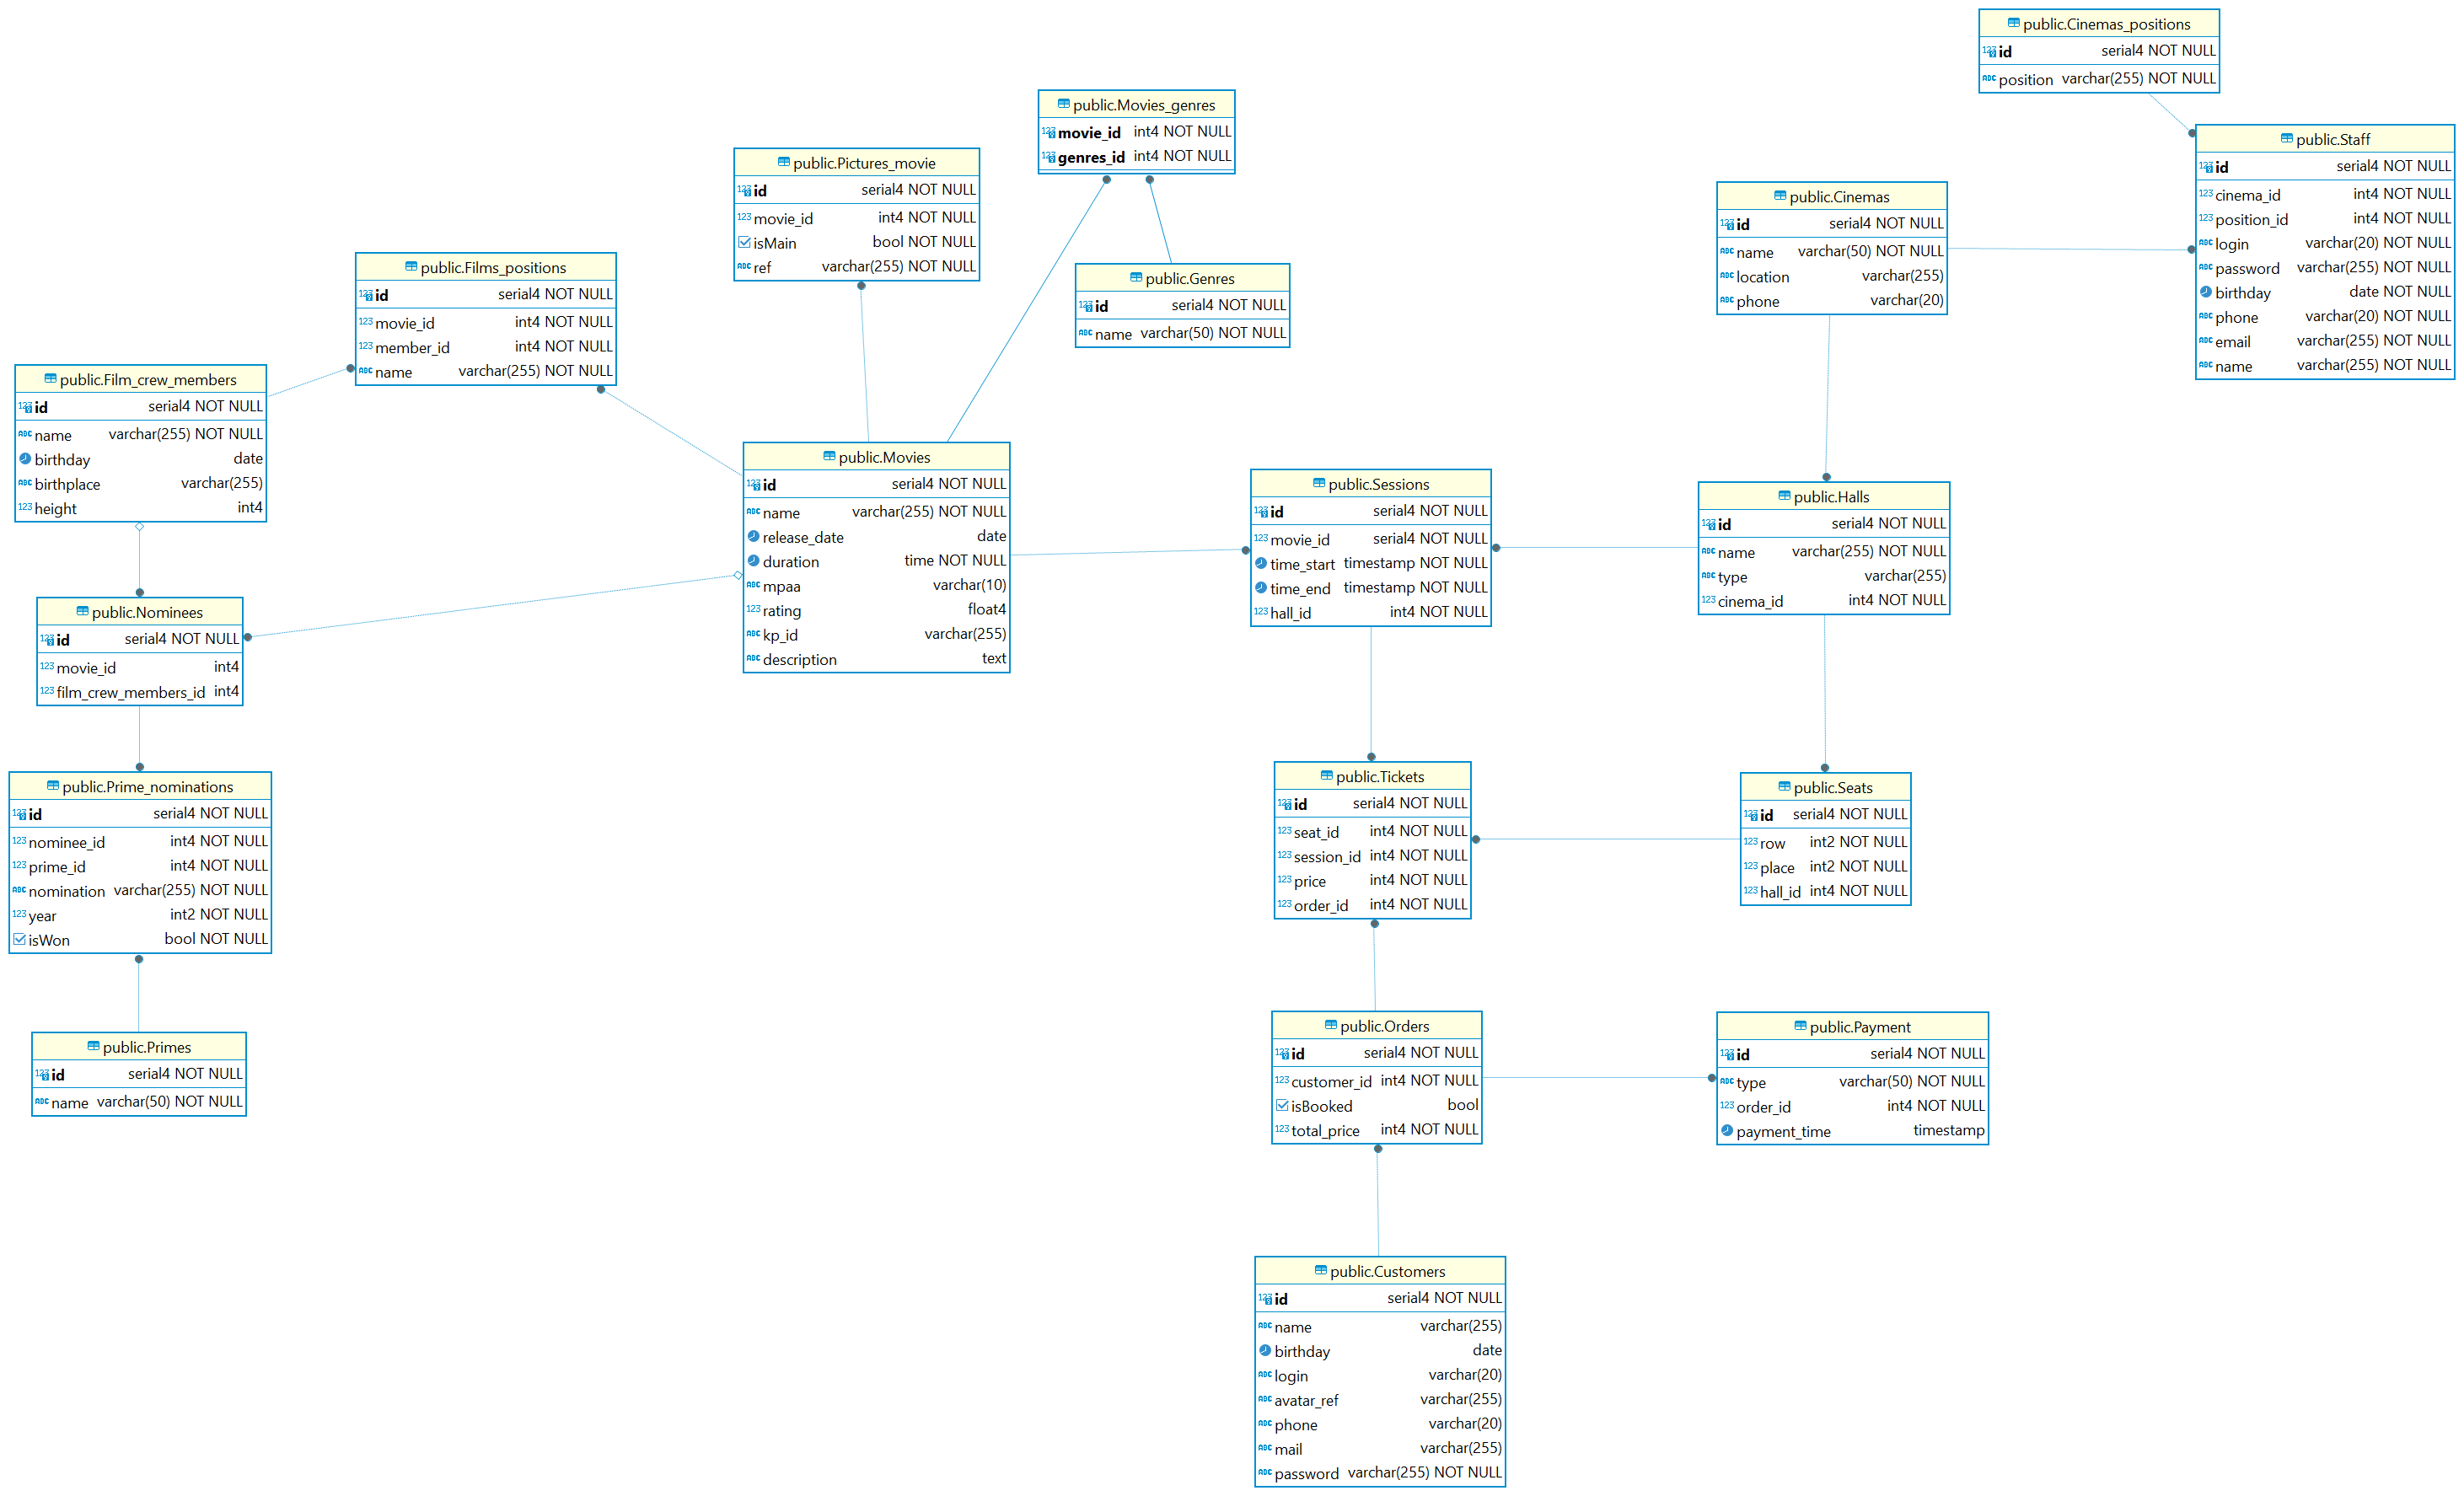
\includegraphics[scale=0.19,page=1]{Логическая_модель}
		\caption{Логическая модель базы данных}\label{fig:figure2}
	\end{figure}
	
	\newpage
	
	\section{Физическое проектирование}\label{sec:-2}

	В качестве СУБД для реализации разработанной базы данных была выбрана PostgreSQL. В связи с проведённым анализом предметной области и была проработана следующая физическая схема базы данных. Она представлена на следующем рисунке:
	
	\begin{figure}[h]
		\hspace{-1.75cm}
		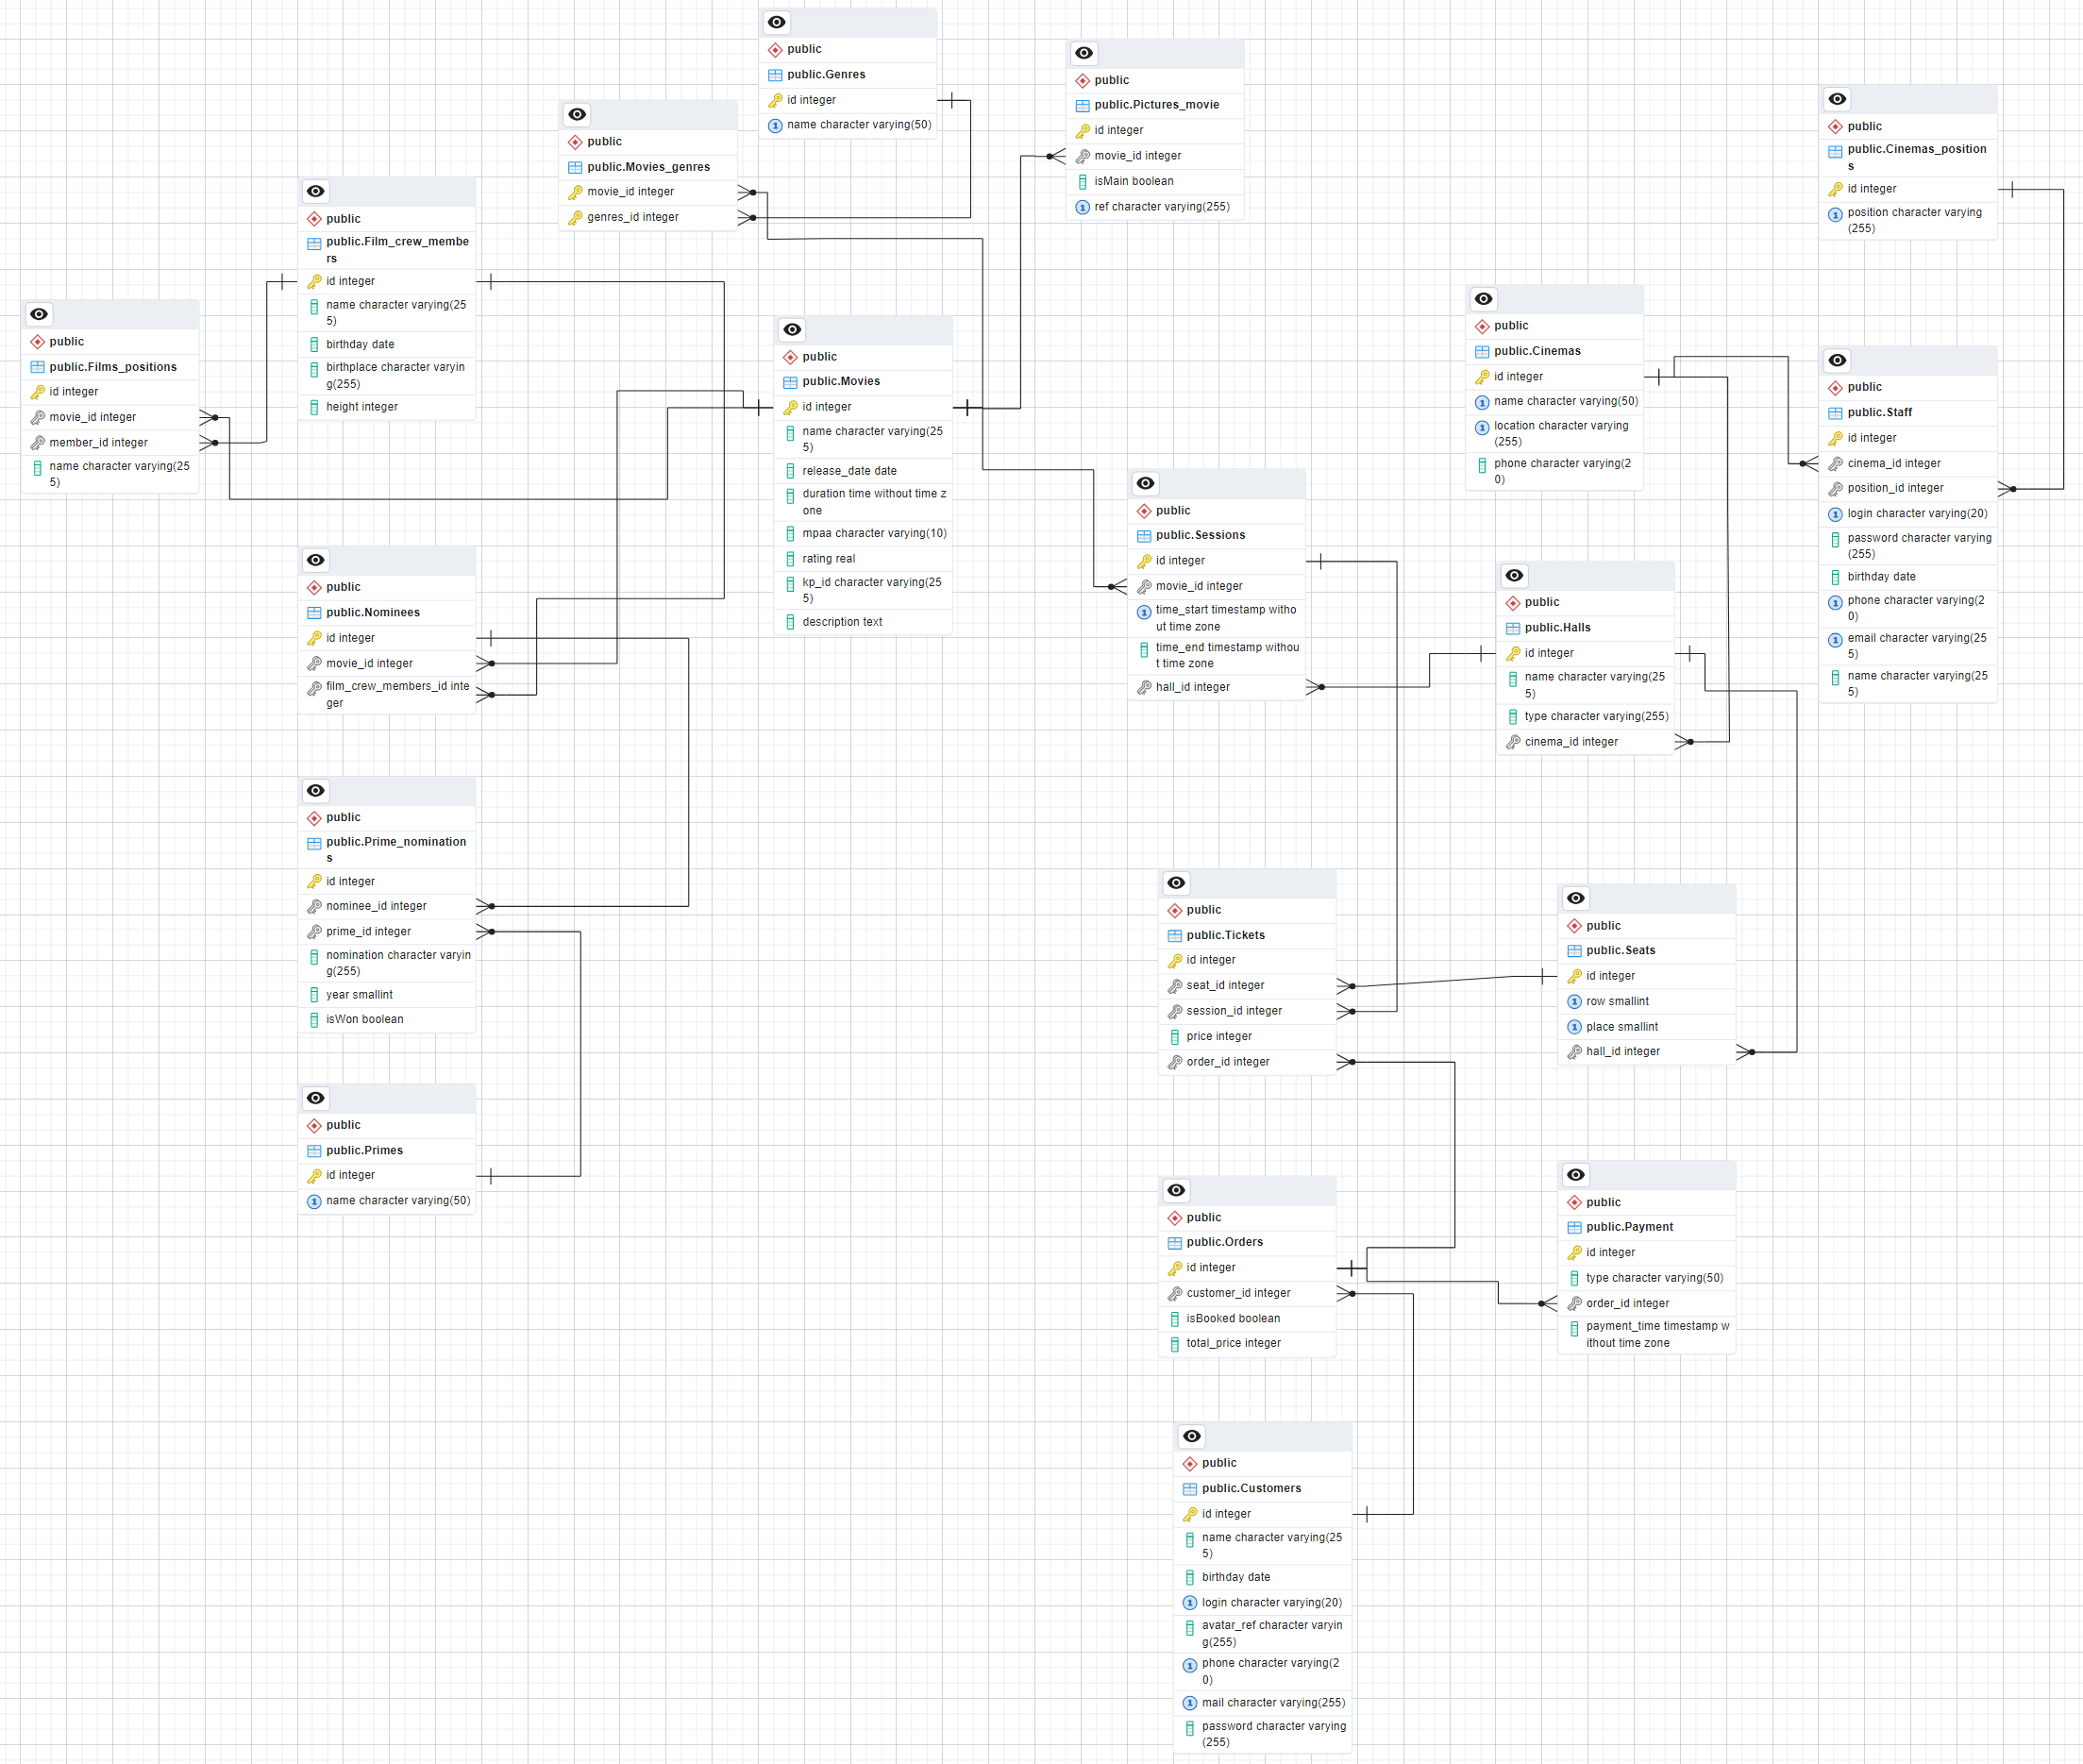
\includegraphics[scale=0.5,page=1]{Графическое_представление}
		\caption{Графическое представление базы данных}\label{fig:figure3}
	\end{figure}
	
	\newpage
	
	\subsection{Создание таблиц}\label{subsec:-}

	Ниже приведены скриптовый код на языке SQL (диалект PostgreSQL) для создания таблиц, описанных выше.
	
	\begin{itemize}
	
	\lstdefinestyle{vscode-dark}{
		backgroundcolor=\color{black},
		basicstyle=\color{white}\ttfamily\fontsize{8}{11}\selectfont,
		breakatwhitespace=false,
		breaklines=true,
		captionpos=b,
		commentstyle=\color{green!40!black},
		keywordstyle=\color{cyan},
		numbersep=5pt,
		numberstyle=\tiny\color{gray},
		showstringspaces=false,
		stringstyle=\color{orange},
		tabsize=4,
		extendedchars=true,
		upquote=true,
		literate=
			{а}{{\selectfont\char224}}1
			{б}{{\selectfont\char225}}1
			{в}{{\selectfont\char226}}1
			{г}{{\selectfont\char227}}1
			{д}{{\selectfont\char228}}1
			{е}{{\selectfont\char229}}1
			{ё}{{\"e}}1
			{ж}{{\selectfont\char230}}1
			{з}{{\selectfont\char231}}1
			{и}{{\selectfont\char232}}1
			{й}{{\selectfont\char233}}1
			{к}{{\selectfont\char234}}1
			{л}{{\selectfont\char235}}1
			{м}{{\selectfont\char236}}1
			{н}{{\selectfont\char237}}1
			{о}{{\selectfont\char238}}1
			{п}{{\selectfont\char239}}1
			{р}{{\selectfont\char240}}1
			{с}{{\selectfont\char241}}1
			{т}{{\selectfont\char242}}1
			{у}{{\selectfont\char243}}1
			{ф}{{\selectfont\char244}}1
			{х}{{\selectfont\char245}}1
			{ц}{{\selectfont\char246}}1
			{ч}{{\selectfont\char247}}1
			{ш}{{\selectfont\char248}}1
			{щ}{{\selectfont\char249}}1
			{ъ}{{\selectfont\char250}}1
			{ы}{{\selectfont\char251}}1
			{ь}{{\selectfont\char252}}1
			{э}{{\selectfont\char253}}1
			{ю}{{\selectfont\char254}}1
			{я}{{\selectfont\char255}}1
			{А}{{\selectfont\char192}}1
			{Б}{{\selectfont\char193}}1
			{В}{{\selectfont\char194}}1
			{Г}{{\selectfont\char195}}1
			{Д}{{\selectfont\char196}}1
			{Е}{{\selectfont\char197}}1
			{Ё}{{\"E}}1
			{Ж}{{\selectfont\char198}}1
			{З}{{\selectfont\char199}}1
			{И}{{\selectfont\char200}}1
			{Й}{{\selectfont\char201}}1
			{К}{{\selectfont\char202}}1
			{Л}{{\selectfont\char203}}1
			{М}{{\selectfont\char204}}1
			{Н}{{\selectfont\char205}}1
			{О}{{\selectfont\char206}}1
			{П}{{\selectfont\char207}}1
			{Р}{{\selectfont\char208}}1
			{С}{{\selectfont\char209}}1
			{Т}{{\selectfont\char210}}1
			{У}{{\selectfont\char211}}1
			{Ф}{{\selectfont\char212}}1
			{Х}{{\selectfont\char213}}1
			{Ц}{{\selectfont\char214}}1
			{Ч}{{\selectfont\char215}}1
			{Ш}{{\selectfont\char216}}1
			{Щ}{{\selectfont\char217}}1
			{Ъ}{{\selectfont\char218}}1
			{Ы}{{\selectfont\char219}}1
			{Ь}{{\selectfont\char220}}1
			{Э}{{\selectfont\char221}}1
			{Ю}{{\selectfont\char222}}1
			{Я}{{\selectfont\char223}}1
	}
	
	\item Код для создания таблицы Movies
		
	\begin{lstlisting}[style=vscode-dark, language=SQL, label={lst:sql}]
		CREATE TABLE IF NOT EXISTS "public.Movies" (
			"id" serial NOT NULL,
			"name" varchar(255) NOT NULL,
			"release_date" DATE,
			"duration" TIME NOT NULL,
			"mpaa" varchar(10),
			"rating" float4,
			"kp_id" varchar(255),
			"description" TEXT,
			CONSTRAINT "Movies_pk" PRIMARY KEY ("id")
		) WITH (
			OIDS=FALSE
		);
	\end{lstlisting}


	\item Код для создания таблицы Genres

	\begin{lstlisting}[style=vscode-dark, language=SQL, label={lst:sql2}]
		CREATE TABLE IF NOT EXISTS "public.Genres" (
			"id" serial NOT NULL,
			"name" varchar(50) UNIQUE NOT NULL,
		CONSTRAINT "Genres_pk" PRIMARY KEY ("id")
		) WITH (
			OIDS=FALSE
		);
	\end{lstlisting}

	\item Код для создания таблицы Movies\_genres

	\begin{lstlisting}[style=vscode-dark, language=SQL, label={lst:sql3}]
		CREATE TABLE IF NOT EXISTS "public.Movies_genres" (
			"movie_id" integer NOT NULL,
			"genres_id" integer NOT NULL,
			CONSTRAINT "Movies_genres_pk" PRIMARY KEY ("movie_id", "genres_id")
		) WITH (
			OIDS=FALSE
		);
		
		ALTER TABLE "public.Movies_genres" ADD CONSTRAINT "Movies_genres_fk0" FOREIGN KEY ("movie_id") REFERENCES "public.Movies"("id");
		ALTER TABLE "public.Movies_genres" ADD CONSTRAINT "Movies_genres_fk1" FOREIGN KEY ("genres_id") REFERENCES "public.Genres"("id");
	\end{lstlisting}

	\item Код для создания таблицы Pictures\_movie

	\begin{lstlisting}[style=vscode-dark, language=SQL, label={lst:sql4}]
		CREATE TABLE IF NOT EXISTS "public.Pictures_movie" (
			"id" serial NOT NULL,
			"movie_id" integer NOT NULL,
			"isMain" BOOLEAN NOT NULL DEFAULT 'false',
			"ref" varchar(255) NOT NULL UNIQUE,
			CONSTRAINT "Pictures_movie_pk" PRIMARY KEY ("id")
		) WITH (
			OIDS=FALSE
		);
		
		ALTER TABLE "public.Pictures_movie" ADD CONSTRAINT "Pictures_movie_fk0" FOREIGN KEY ("movie_id") REFERENCES "public.Movies"("id");
	\end{lstlisting}
	%$\\$
	
	\item Код для создания таблицы Film\_crew\_members
	
	\begin{lstlisting}[style=vscode-dark, language=SQL, label={lst:sql5}]
		CREATE TABLE IF NOT EXISTS "public.Film_crew_members" (
			"id" serial NOT NULL,
			"name" varchar(255) NOT NULL,
			"birthday" DATE,
			"birthplace" varchar(255),
			"height" integer,
			CONSTRAINT "Film_crew_members_pk" PRIMARY KEY ("id")
		) WITH (
			OIDS=FALSE
		);
	\end{lstlisting}

	\item Код для создания таблицы Films\_positions

	\begin{lstlisting}[style=vscode-dark, language=SQL, label={lst:sql6}]
		CREATE TABLE IF NOT EXISTS "public.Films_positions" (
			"id" serial NOT NULL,
			"movie_id" integer NOT NULL,
			"member_id" integer NOT NULL,
			"name" varchar(255) NOT NULL,
			CONSTRAINT "Films_crews_pk" PRIMARY KEY ("id")
		) WITH (
			OIDS=FALSE
		);
		
		ALTER TABLE "public.Films_positions" ADD CONSTRAINT "Films_positions_fk0" FOREIGN KEY ("movie_id") REFERENCES "public.Movies"("id");
		ALTER TABLE "public.Films_positions" ADD CONSTRAINT "Films_positions_fk1" FOREIGN KEY ("member_id") REFERENCES "public.Film_crew_members"("id");
	\end{lstlisting}
	\newpage
	
	\item Код для создания таблицы Nominees
	
	\begin{lstlisting}[style=vscode-dark, language=SQL, label={lst:sql7}]
		CREATE TABLE IF NOT EXISTS "public.Nominees" (
			"id" serial NOT NULL,
			"movie_id" integer,
			"film_crew_members_id" integer,
			CONSTRAINT "Nominees_pk" PRIMARY KEY ("id")
		) WITH (
			OIDS=FALSE
		);
		
		ALTER TABLE "public.Nominees" ADD CONSTRAINT "Nominees_fk0" FOREIGN KEY ("movie_id") REFERENCES "public.Movies"("id");
		ALTER TABLE "public.Nominees" ADD CONSTRAINT "Nominees_fk1" FOREIGN KEY ("film_crew_members_id") REFERENCES "public.Film_crew_members"("id");
		ALTER TABLE "public.Nominees" ADD CONSTRAINT "Nominees_unique" UNIQUE("movie_id","film_crew_members_id");
	\end{lstlisting}
	
	\item Код для создания таблицы Primes
	
	\begin{lstlisting}[style=vscode-dark, language=SQL, label={lst:sql8}]
		CREATE TABLE IF NOT EXISTS "public.Primes" (
			"id" serial NOT NULL,
			"name" varchar(50) NOT NULL UNIQUE,
			CONSTRAINT "Primes_pk" PRIMARY KEY ("id")
		) WITH (
			OIDS=FALSE
		);
	\end{lstlisting}

	\item Код для создания таблицы Prime\_nominations

	\begin{lstlisting}[style=vscode-dark, language=SQL, label={lst:sql9}]
		CREATE TABLE IF NOT EXISTS "public.Prime_nominations" (
			"id" serial NOT NULL,
			"nominee_id" integer NOT NULL,
			"prime_id" integer NOT NULL,
			"nomination" varchar(255) NOT NULL,
			"year" smallint NOT NULL,
			"isWon" BOOLEAN NOT NULL DEFAULT 'false',
			CONSTRAINT "Prime_nominations_pk" PRIMARY KEY ("id")
		) WITH (
			OIDS=FALSE
		);
		
		ALTER TABLE "public.Prime_nominations" ADD CONSTRAINT "Prime_nominations_fk0" FOREIGN KEY ("nominee_id") REFERENCES "public.Nominees"("id");
		ALTER TABLE "public.Prime_nominations" ADD CONSTRAINT "Prime_nominations_fk1" FOREIGN KEY ("prime_id") REFERENCES "public.Primes"("id");
	\end{lstlisting}
	
	\item Код для создания таблицы Cinemas
	
	\begin{lstlisting}[style=vscode-dark, language=SQL, label={lst:sql10}]
		CREATE TABLE IF NOT EXISTS "public.Cinemas" (
			"id" serial NOT NULL,
			"name" varchar(50) NOT NULL UNIQUE,
			"location" varchar(255) UNIQUE,
			"phone" varchar(20),
			CONSTRAINT "Cinemas_pk" PRIMARY KEY ("id")
		) WITH (
			OIDS=FALSE
		);
	\end{lstlisting}
	
	\item Код для создания таблицы Halls
	
	\begin{lstlisting}[style=vscode-dark, language=SQL, label={lst:sql11}]
		CREATE TABLE IF NOT EXISTS "public.Halls" (
			"id" serial NOT NULL,
			"name" varchar(255) NOT NULL,
			"type" varchar(255),
			"cinema_id" integer NOT NULL,
			CONSTRAINT "Halls_pk" PRIMARY KEY ("id")
		) WITH (
			OIDS=FALSE
		);
		
		ALTER TABLE "public.Halls" ADD CONSTRAINT "Halls_fk0" FOREIGN KEY ("cinema_id") REFERENCES "public.Cinemas"("id");
	\end{lstlisting}

	\item Код для создания таблицы Sessions

	\begin{lstlisting}[style=vscode-dark, language=SQL, label={lst:sql12}]
		CREATE TABLE IF NOT EXISTS "public.Sessions" (
			"id" serial NOT NULL,
			"movie_id" serial NOT NULL ,
			"time_start" TIMESTAMP NOT NULL,
			"time_end" TIMESTAMP NOT NULL,
			"hall_id" integer NOT NULL,
			CONSTRAINT "Sessions_pk" PRIMARY KEY ("id")
		) WITH (
			OIDS=FALSE
		);
		
		ALTER TABLE "public.Sessions" ADD CONSTRAINT "Sessions_fk0" FOREIGN KEY ("movie_id") REFERENCES "public.Movies"("id");
		ALTER TABLE "public.Sessions" ADD CONSTRAINT "Sessions_fk1" FOREIGN KEY ("hall_id") REFERENCES "public.Halls"("id");
		ALTER TABLE "public.Sessions" ADD CONSTRAINT "Sessions_unique" UNIQUE("hall_id", "time_start");
	\end{lstlisting}
	
	\item Код для создания таблицы Seats
	
	\begin{lstlisting}[style=vscode-dark, language=SQL, label={lst:sql13}]
		CREATE TABLE IF NOT EXISTS "public.Seats" (
			"id" serial NOT NULL,
			"row" smallint NOT NULL,
			"place" smallint NOT NULL,
			"hall_id" integer NOT NULL,
			CONSTRAINT "Seats_pk" PRIMARY KEY ("id")
		) WITH (
			OIDS=FALSE
		);
		
		ALTER TABLE "public.Seats" ADD CONSTRAINT "Seats_fk0" FOREIGN KEY ("hall_id") REFERENCES "public.Halls"("id");
		ALTER TABLE "public.Seats" ADD CONSTRAINT "Seats_unique" UNIQUE("row", "place", "hall_id");
	\end{lstlisting}

	\item Код для создания таблицы Customers

	\begin{lstlisting}[style=vscode-dark, language=SQL, label={lst:sql14}]
		CREATE TABLE IF NOT EXISTS "public.Customers" (
			"id" serial NOT NULL,
			"name" varchar(255),
			"birthday" DATE,
			"login" varchar(20) UNIQUE,
			"avatar_ref" varchar(255),
			"phone" varchar(20) UNIQUE,
			"mail" varchar(255) UNIQUE,
			"password" varchar(255) NOT NULL,
			CONSTRAINT "Customers_pk" PRIMARY KEY ("id")
		) WITH (
			OIDS=FALSE
		);
	\end{lstlisting}

	\item Код для создания таблицы Orders

	\begin{lstlisting}[style=vscode-dark, language=SQL, label={lst:sql15}]
		CREATE TABLE IF NOT EXISTS "public.Orders" (
			"id" serial NOT NULL,
			"customer_id" integer NOT NULL,
			"isBooked" BOOLEAN DEFAULT(false),
			"total_price" integer NOT NULL DEFAULT 0,
			CONSTRAINT "Orders_pk" PRIMARY KEY ("id")
		) WITH (
			OIDS=FALSE
		);
		
		ALTER TABLE "public.Orders" ADD CONSTRAINT "Orders_fk0" FOREIGN KEY ("customer_id") REFERENCES "public.Customers"("id");
	\end{lstlisting}
	
	\item Код для создания таблицы Payment

	\begin{lstlisting}[style=vscode-dark, language=SQL, label={lst:sql16}]
		CREATE TABLE IF NOT EXISTS "public.Payment" (
			"id" serial NOT NULL,
			"type" varchar(50) NOT NULL,
			"order_id" integer NOT NULL UNIQUE,
			"payment_time" TIMESTAMP,
			CONSTRAINT "Payment_pk" PRIMARY KEY ("id")
		) WITH (
			OIDS=FALSE
		);
		
		ALTER TABLE "public.Payment"  ADD CONSTRAINT "Payment_fk0" FOREIGN KEY ("order_id") REFERENCES "public.Orders"("id");
	\end{lstlisting}

	\item Код для создания таблицы Tickets

	\begin{lstlisting}[style=vscode-dark, language=SQL, label={lst:sql17}]
		CREATE TABLE IF NOT EXISTS "public.Tickets" (
			"id" serial NOT NULL,
			"seat_id" integer NOT NULL,
			"session_id" integer NOT NULL,
			"price" integer NOT NULL,
			"order_id" integer NOT NULL,
			CONSTRAINT "Tickets_pk" PRIMARY KEY ("id")
		) WITH (
			OIDS=FALSE
		);
		
		ALTER TABLE "public.Tickets" ADD CONSTRAINT "Tickets_fk0" FOREIGN KEY ("seat_id") REFERENCES "public.Seats"("id");
		ALTER TABLE "public.Tickets" ADD CONSTRAINT "Tickets_fk1" FOREIGN KEY ("session_id") REFERENCES "public.Sessions"("id");
		ALTER TABLE "public.Tickets" ADD CONSTRAINT "Tickets_fk2" FOREIGN KEY ("order_id") REFERENCES "public.Orders"("id");
		ALTER TABLE "public.Tickets" ADD CONSTRAINT "Tickets_unique" UNIQUE("seat_id", "session_id");
	\end{lstlisting}
	\newpage

	\item Код для создания таблицы Cinemas\_positions

	\begin{lstlisting}[style=vscode-dark, language=SQL, label={lst:sql18}]
		CREATE TABLE IF NOT EXISTS "public.Cinemas_positions" (
			"id" serial NOT NULL,
			"position" varchar(255) NOT NULL UNIQUE,
			CONSTRAINT "Cinemas_positions_pk" PRIMARY KEY ("id")
		) WITH (
			OIDS=FALSE
		);
	\end{lstlisting}
	
	\item Код для создания таблицы Staff
	
	\begin{lstlisting}[style=vscode-dark, language=SQL, label={lst:sql19}]
		CREATE TABLE IF NOT EXISTS "public.Staff" (
			"id" serial NOT NULL,
			"cinema_id" integer NOT NULL,
			"position_id" integer NOT NULL,
			"login" varchar(20) NOT NULL UNIQUE,
			"password" varchar(255) NOT NULL,
			"birthday" DATE NOT NULL,
			"phone" varchar(20) NOT NULL UNIQUE,
			"email" varchar(255) NOT NULL UNIQUE,
			"name" varchar(255) NOT NULL,
		CONSTRAINT "Staff_pk" PRIMARY KEY ("id")
		) WITH (
			OIDS=FALSE
		);
		
		ALTER TABLE "public.Staff" ADD CONSTRAINT "Staff_fk0" FOREIGN KEY ("cinema_id") REFERENCES "public.Cinemas"("id");
		ALTER TABLE "public.Staff" ADD CONSTRAINT "Staff_fk1" FOREIGN KEY ("position_id") REFERENCES "public.Cinemas_positions"("id");
	\end{lstlisting}

	\end{itemize}
		
		
	\newpage
	
	\subsection{Заполнение базы данных}\label{subsec:--}

	%\newpage
	
	\subsubsection{Подготовка данных}
	
	В сети Интернет найдены такие данные как существующие жанры фильмов, существующие награды и номинации к фильмам. Такие данные как сведения о фильмах (название, дата выхода, длительность, описание), сведения об актёрах (имя, дата рождения, место рождения, рост), сведения о пользователях и сотрудниках (имя, дата рождения, логин, пароль, телефон, почта, ссылка на аватар) были сгенерированы Pyhton библиотекой Faker. Для предварительной оценки сгенерированных данных они были вносились в Excel-таблицы, которые после импортировались в Python с использованием библиотеки Pandas и использовались в автоматизированном написании нужных запросов для заполнения таблиц.
	
	\begin{itemize}
	
	\item Фрагмент сгенерированной Excel-таблицы для заполнения Movies
	
	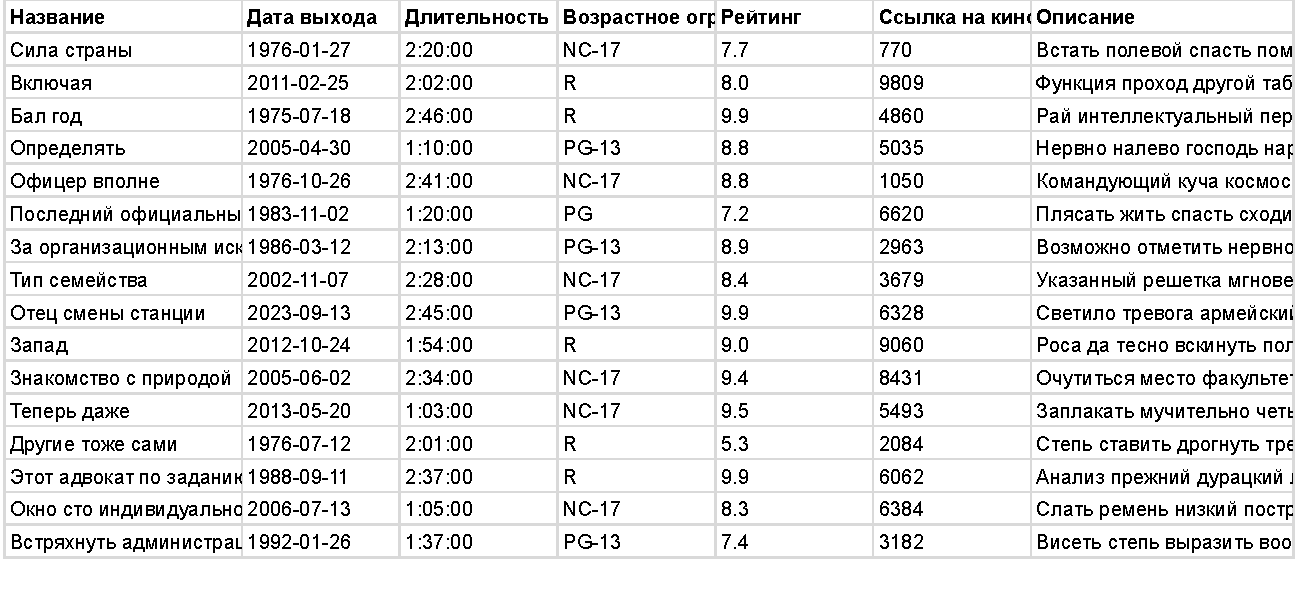
\includegraphics[scale=0.7,page=1]{table_inserts_excel/movies_random}
	

	\item Фрагмент сгенерированной Excel-таблицы для заполнения Movies\_genres
	
	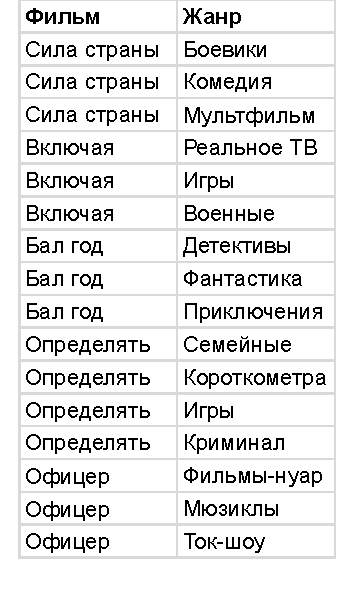
\includegraphics[scale=0.7,page=1]{table_inserts_excel/movies_genres_random}
	

	\item Фрагмент сгенерированной Excel-таблицы для заполнения Pictures\_movie
	
	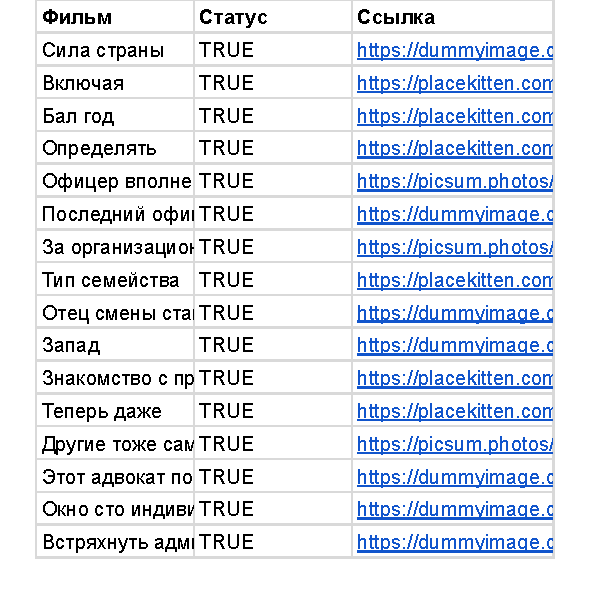
\includegraphics[scale=0.7,page=1]{table_inserts_excel/movie_pictures_random}
	

	\item Фрагмент сгенерированной Excel-таблицы для заполнения Film\_crew\_members
	
	
	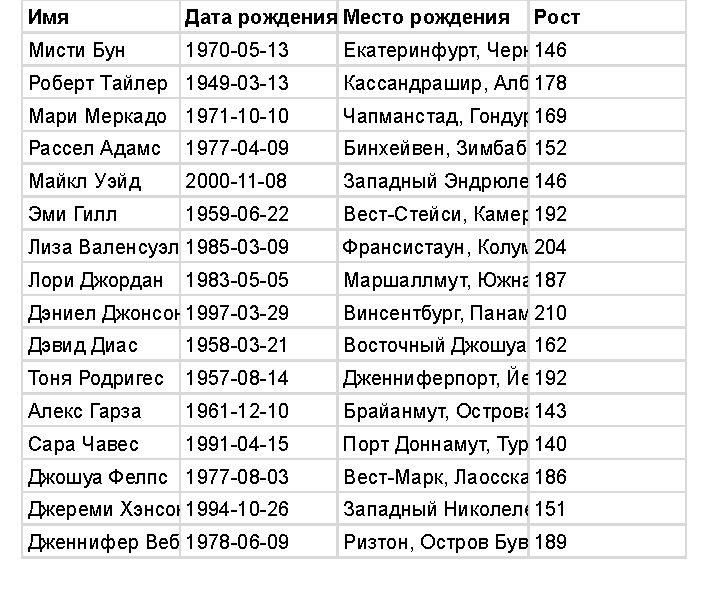
\includegraphics[scale=0.7,page=1]{table_inserts_excel/members_random}
	

	\item Фрагмент сгенерированной Excel-таблицы для заполнения Films\_positions
	
	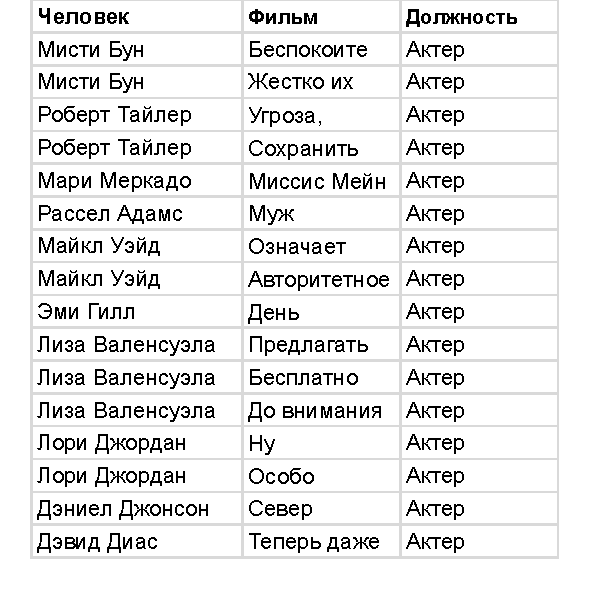
\includegraphics[scale=0.7,page=1]{table_inserts_excel/members_movies_random}
	$\\$
	
	\item Фрагмент сгенерированной Excel-таблицы для заполнения Prime\_nominations
	
	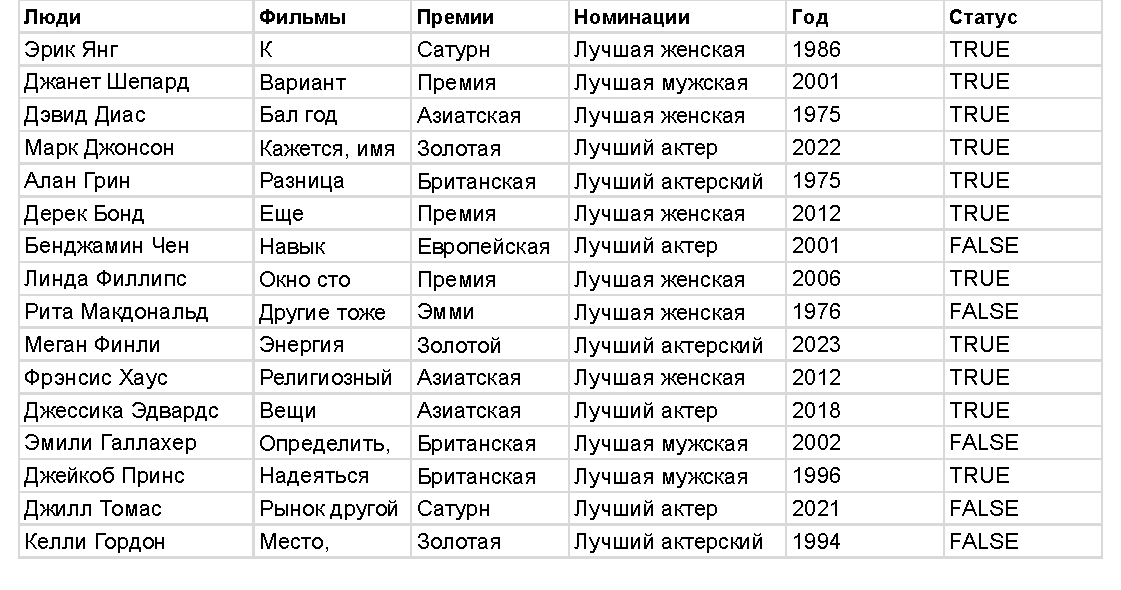
\includegraphics[scale=0.7,page=1]{table_inserts_excel/prime_nominations_random}
	

	\item Фрагмент сгенерированной Excel-таблицы для заполнения Cinemas
	
	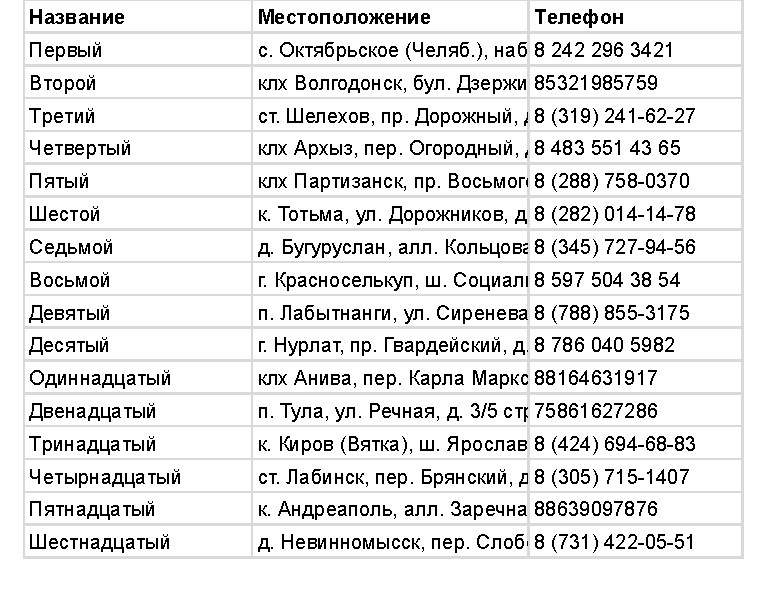
\includegraphics[scale=0.7,page=1]{table_inserts_excel/cinemas_random}
	

	\item Фрагмент сгенерированной Excel-таблицы для заполнения Halls
	
	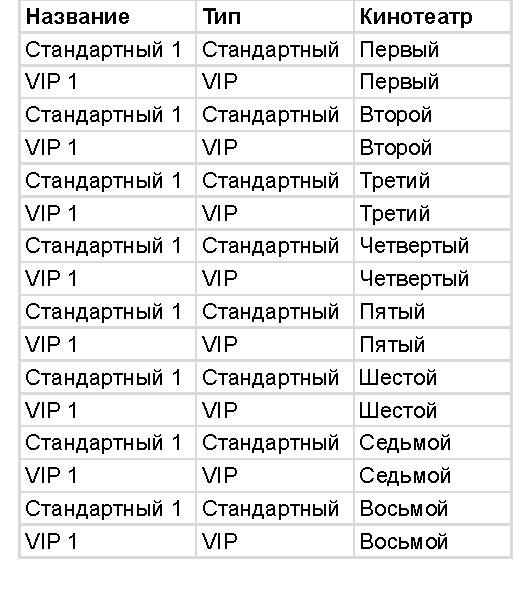
\includegraphics[scale=0.7,page=1]{table_inserts_excel/halls_random}
	$\\$
	
	\item Фрагмент сгенерированной Excel-таблицы для заполнения Sessions
	
	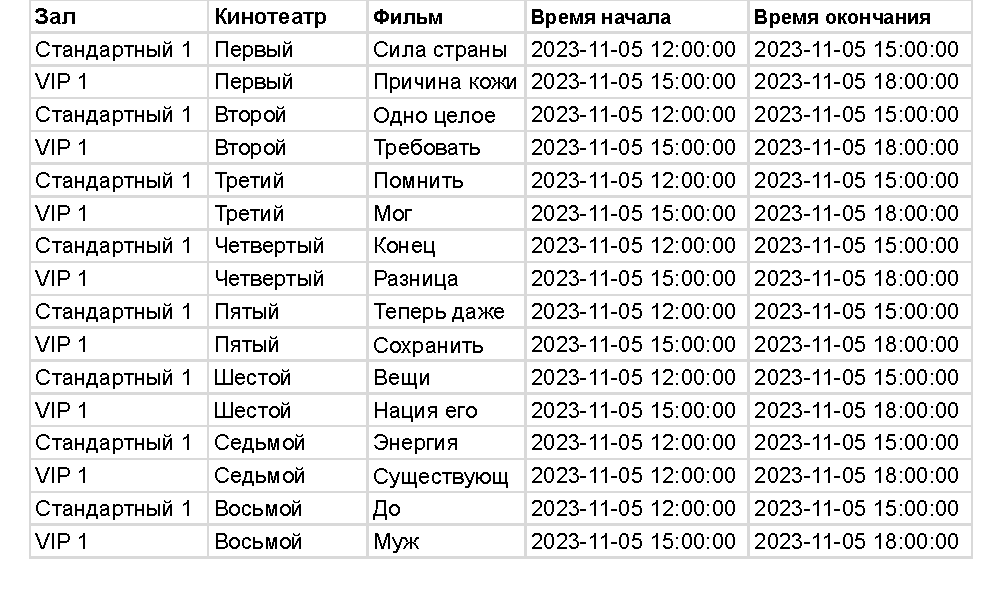
\includegraphics[scale=0.7,page=1]{table_inserts_excel/sessions_random}
	
	
	\item Фрагмент сгенерированной Excel-таблицы для заполнения Customers
	
	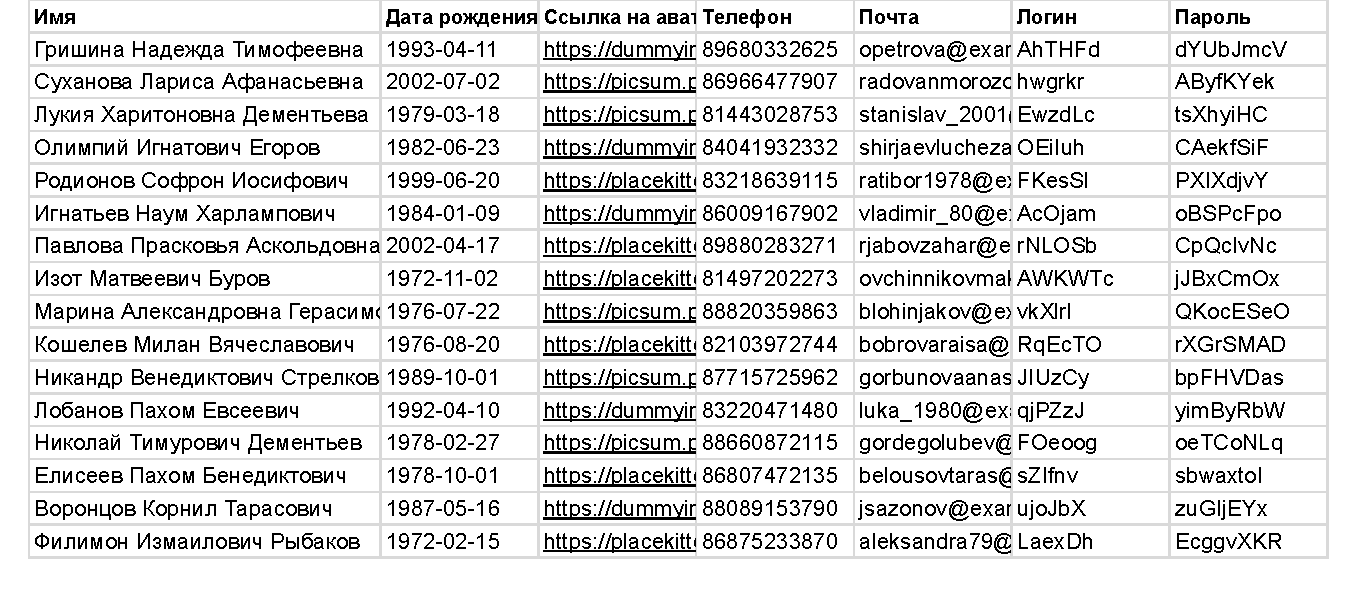
\includegraphics[scale=0.7,page=1]{table_inserts_excel/customers_random}
	
	
	\item Фрагмент сгенерированной Excel-таблицы для заполнения Payment
	
	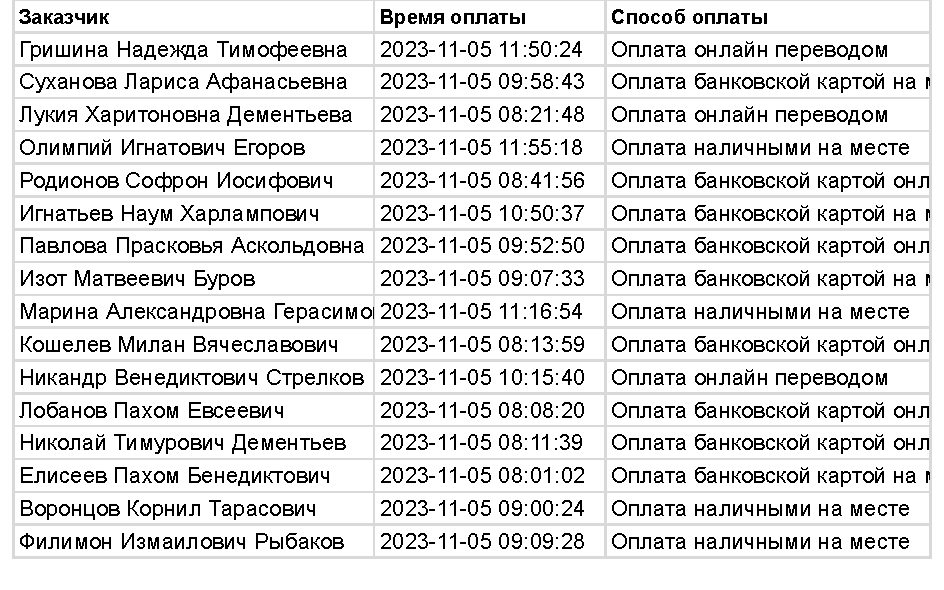
\includegraphics[scale=0.7,page=1]{table_inserts_excel/payment_random}
	$\\$
	
	
	\item Фрагмент сгенерированной Excel-таблицы для заполнения Tickets
	
	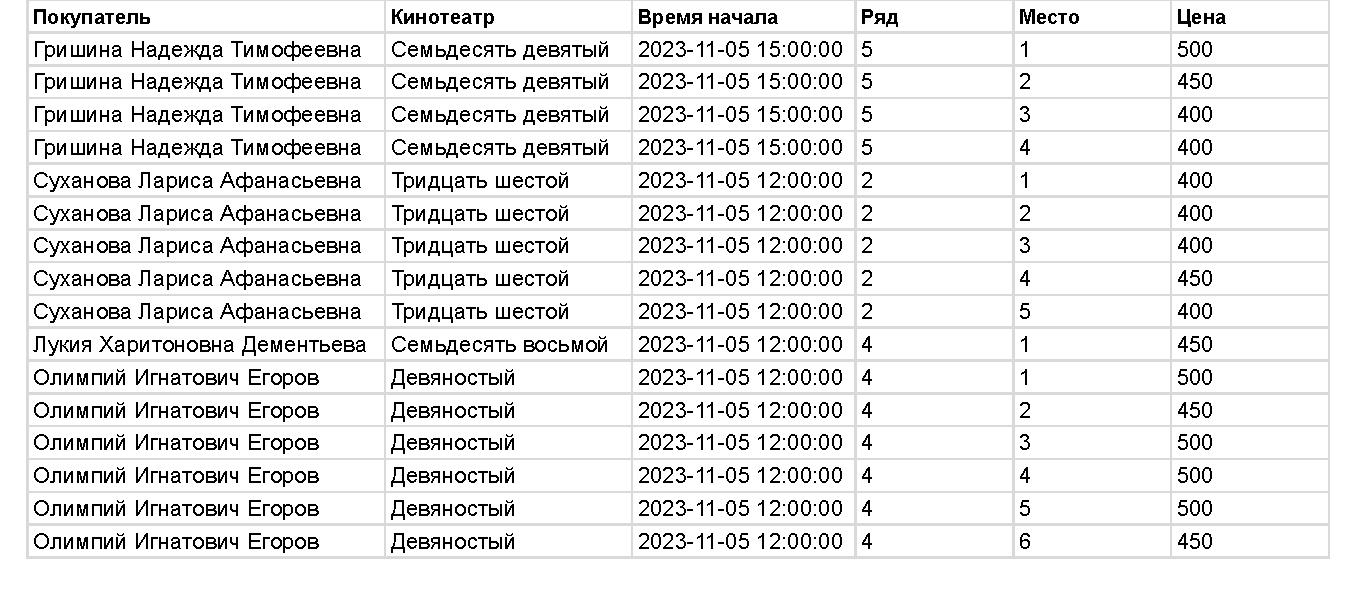
\includegraphics[scale=0.7,page=1]{table_inserts_excel/tickets_random}
	
	
	\item Фрагмент сгенерированной Excel-таблицы для заполнения Staff
	
	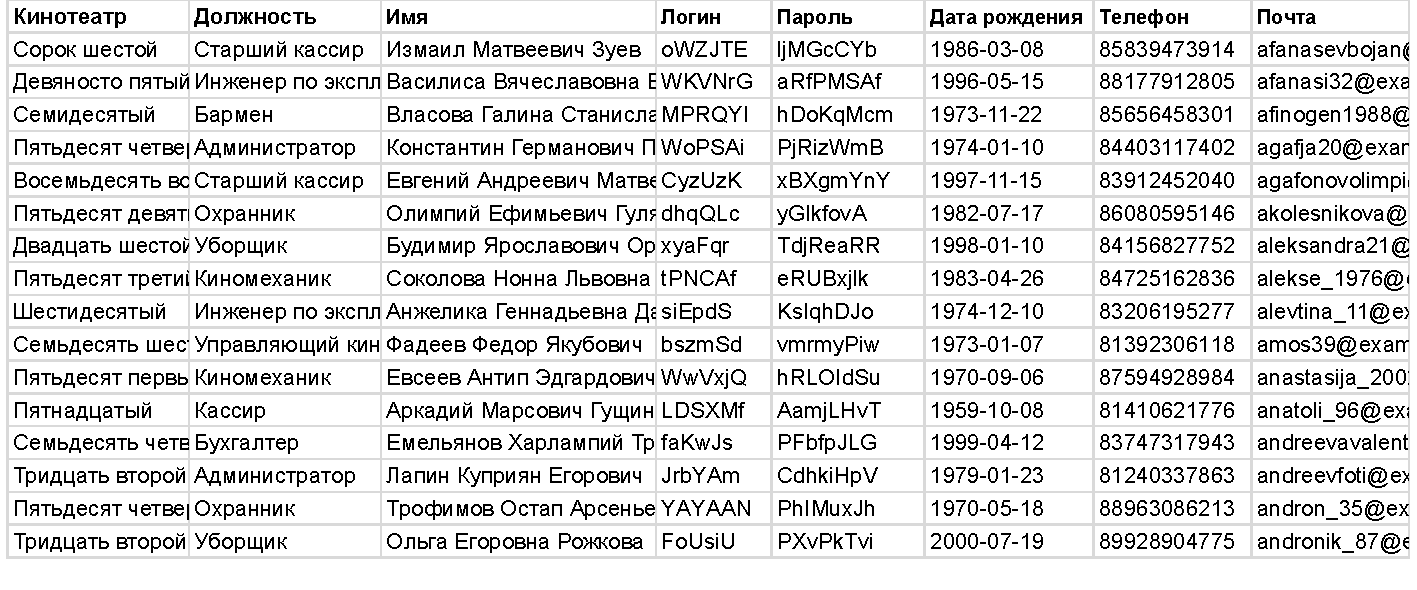
\includegraphics[scale=0.7,page=1]{table_inserts_excel/staff_random}
	
	\end{itemize}
	
	\newpage
	
	\subsubsection{Программа заполнения базы данных}
	
	Ниже приведён пример Python-кода, который принимает данные из Excel-таблицы и генерирует SQL-запрос на заполнение данными таблицы Tickets.
	
	\begin{figure}[h]
		\hspace{-0.5cm}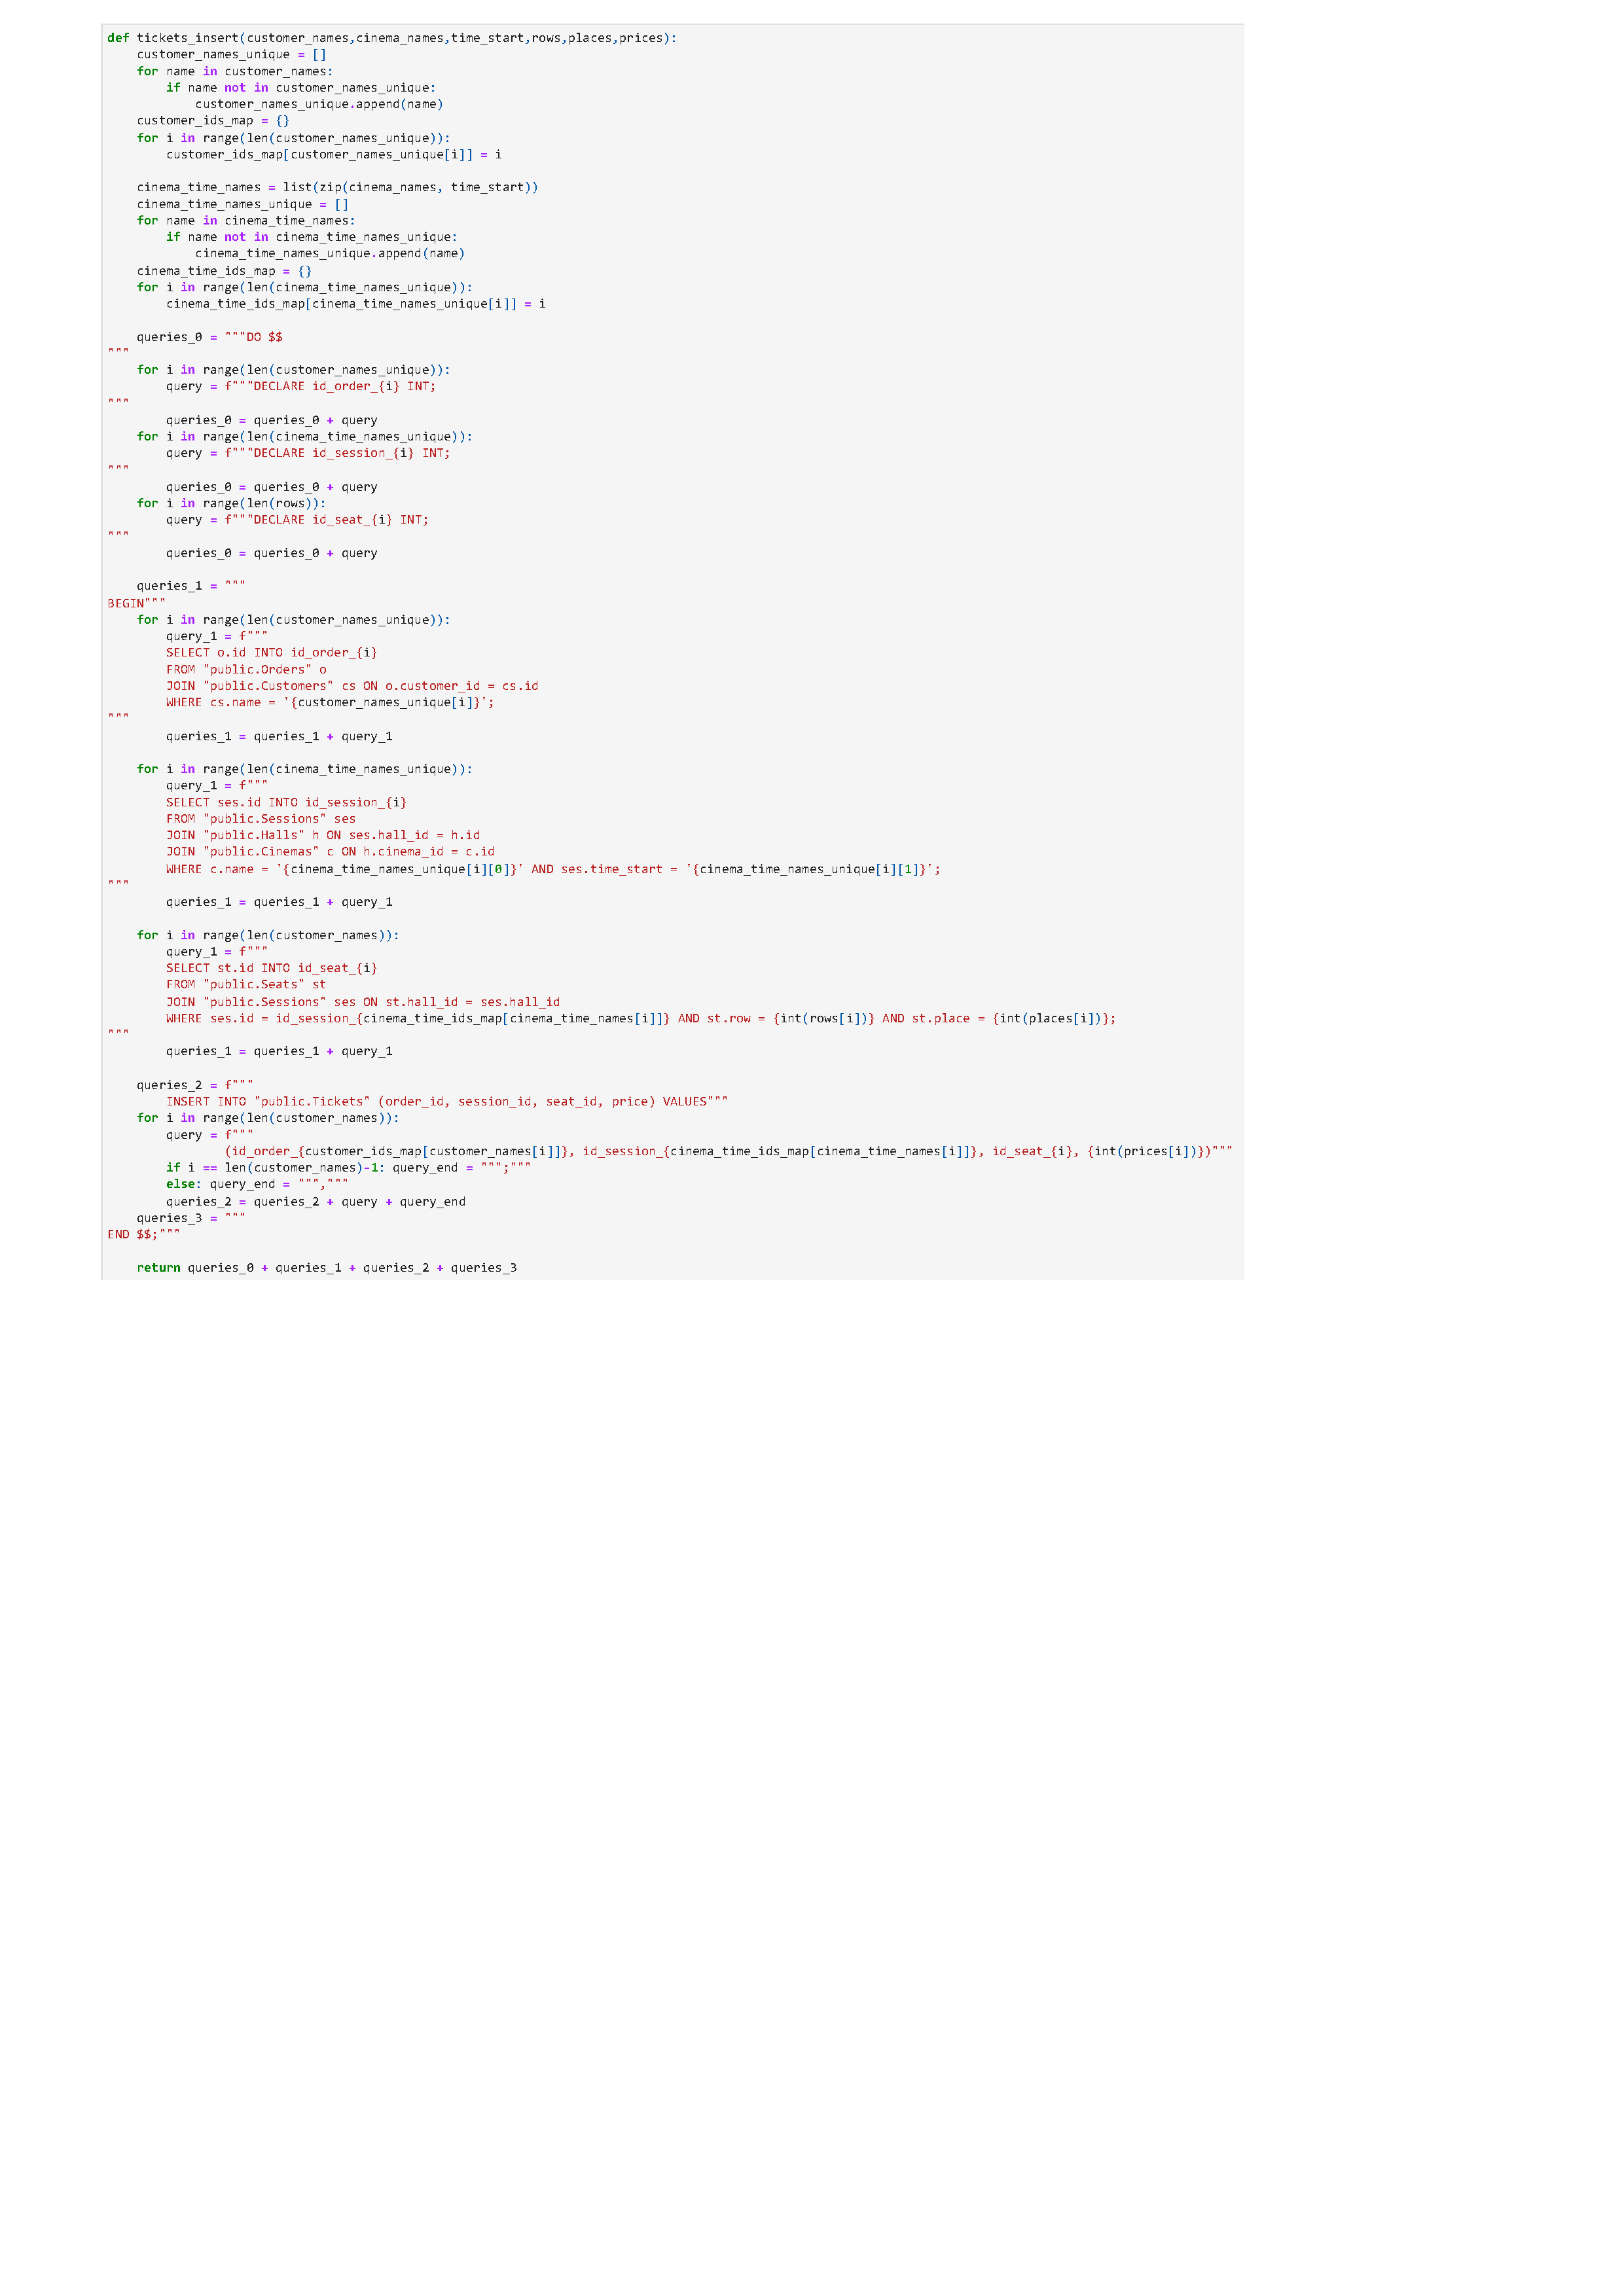
\includegraphics[scale=0.6,page=1]{table_inserts_excel/sql_tickets_insert}\label{fig:figure4}
	\end{figure}

	Все генерируемые подобным образом SQL-запросы направлены на то, чтобы искать id нужных таблиц и заполнять нужные данные на основе данных из Excel-таблиц. Причём нужные id в таком запросе ищутся ровно один раз даже в случае, если в Excel-таблице на один и тот же id ссылаются несколько раз.
	
	\newpage
	
	\subsubsection{Результаты заполнения}
	
	\begin{itemize}
		
	\item Фрагмент таблицы Movies

	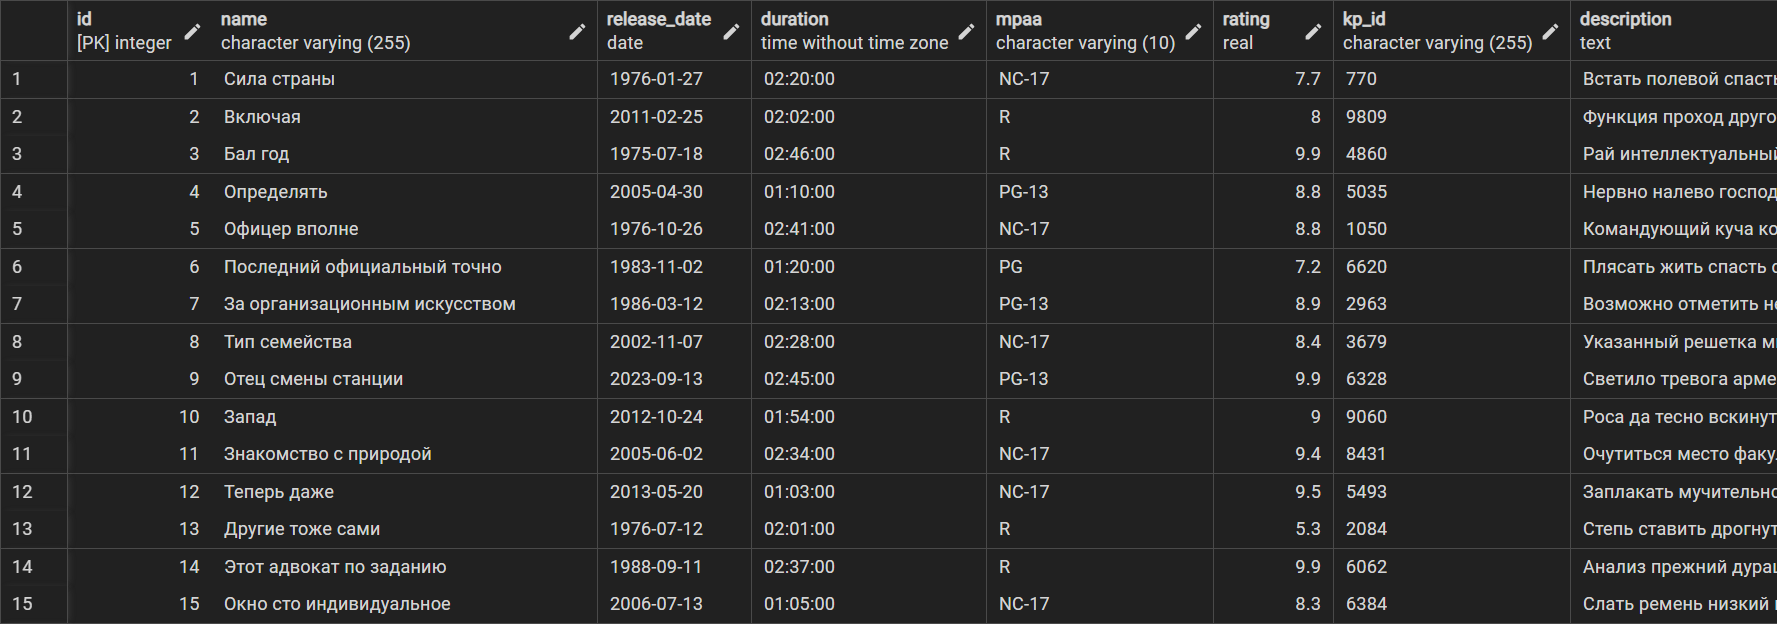
\includegraphics[scale=0.55,page=1]{table_inserts_examples/Movies}
	
	
	\item Таблица Genres
	
	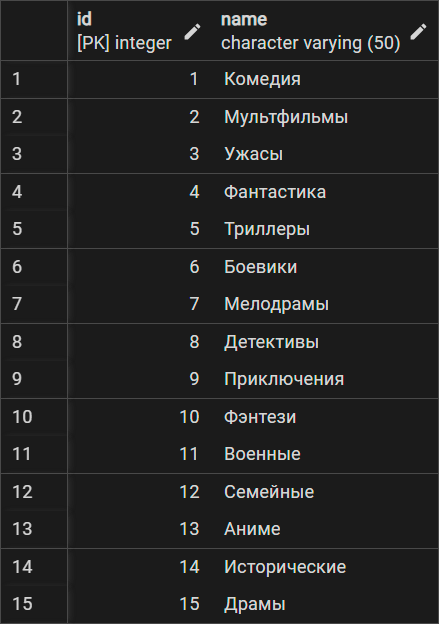
\includegraphics[scale=0.3,page=1]{table_inserts_examples/Genres}
	
	
	\item Фрагмент таблицы Movies\_genres
	
	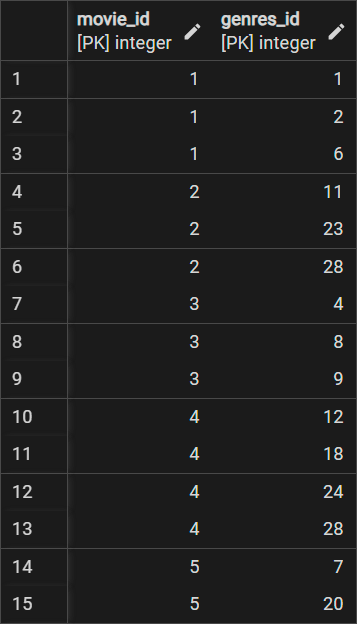
\includegraphics[scale=0.3,page=1]{table_inserts_examples/Movies_genres}
	
	\newpage
	
	
	\item Таблица Pictures\_movie
	
	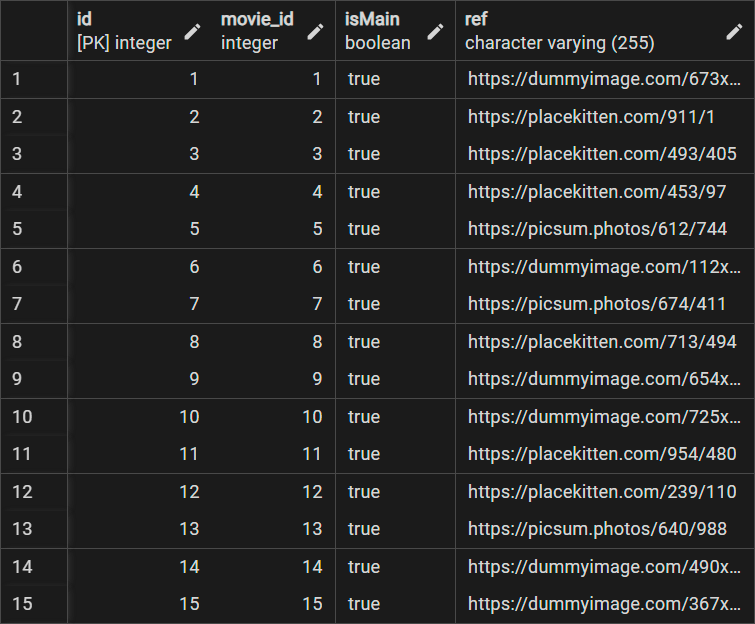
\includegraphics[scale=0.3,page=1]{table_inserts_examples/Pictures_movie}
	
	
	\item Фрагмент таблицы Film\_crew\_members
	
	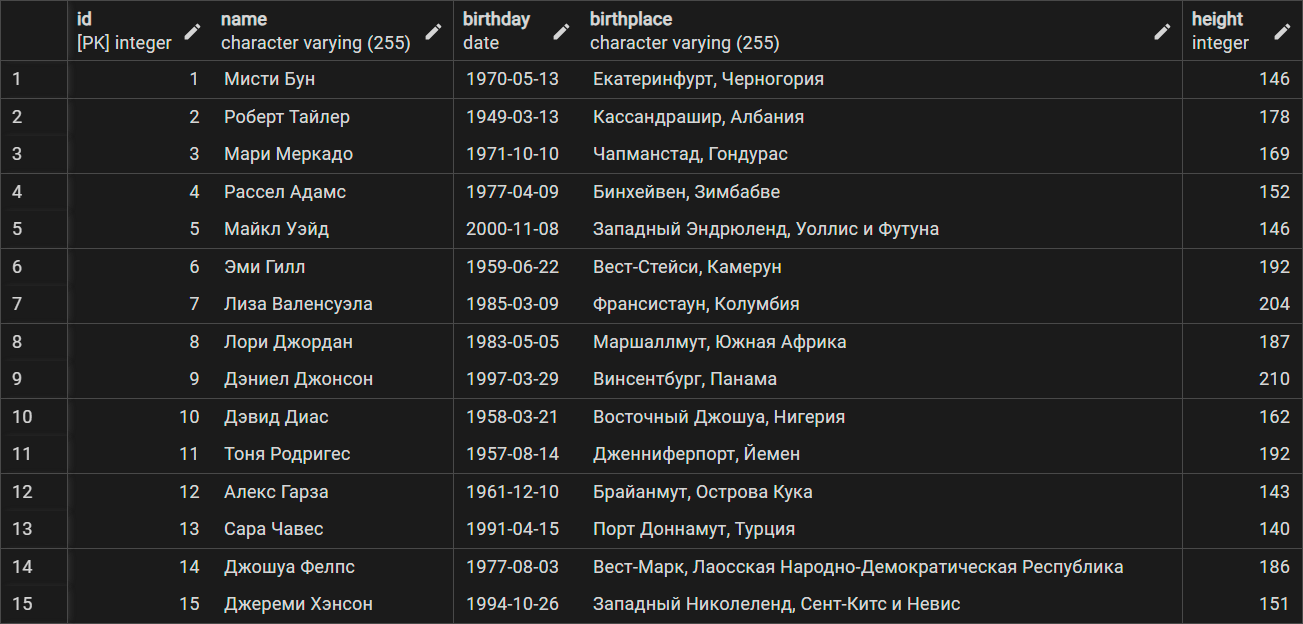
\includegraphics[scale=0.3,page=1]{table_inserts_examples/Film_crew_members}
	
	
	\item Фрагмент таблицы Films\_positions
	
	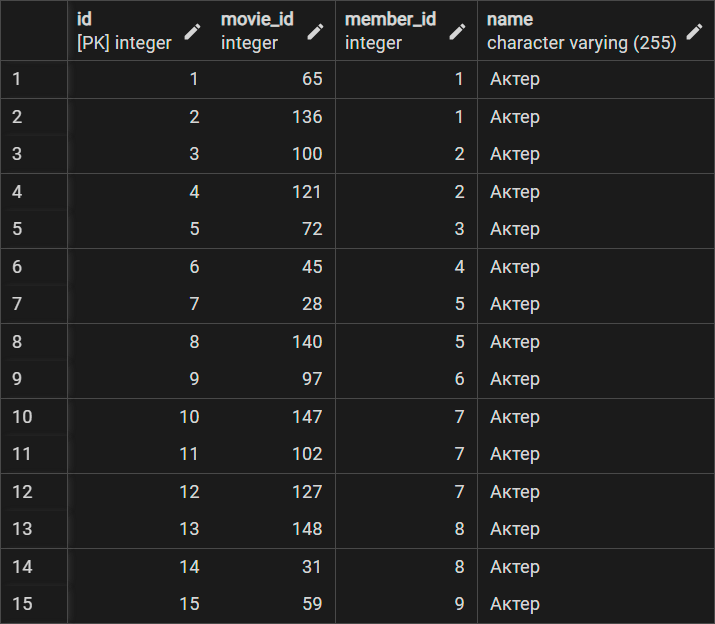
\includegraphics[scale=0.3,page=1]{table_inserts_examples/Films_positions}
	
	\newpage
	
	\item Фрагмент таблицы Nominees
	
	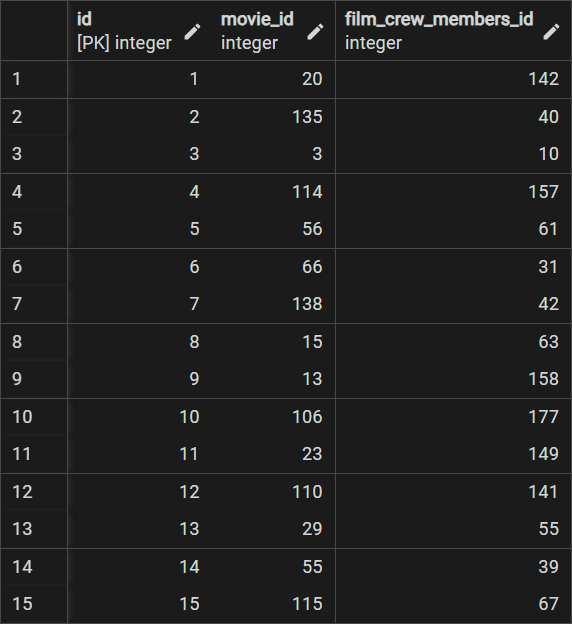
\includegraphics[scale=0.3,page=1]{table_inserts_examples/Nominees}
	$\\$
	
	
	\item Таблица Primes
	
	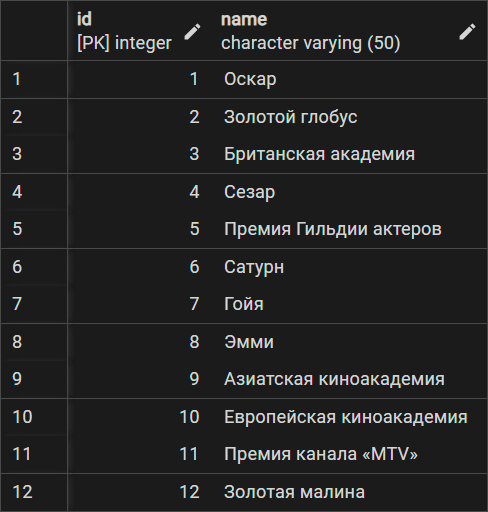
\includegraphics[scale=0.4,page=1]{table_inserts_examples/Primes}
	$\\$
	
	
	\item Фрагмент таблицы Prime\_nominations
	
	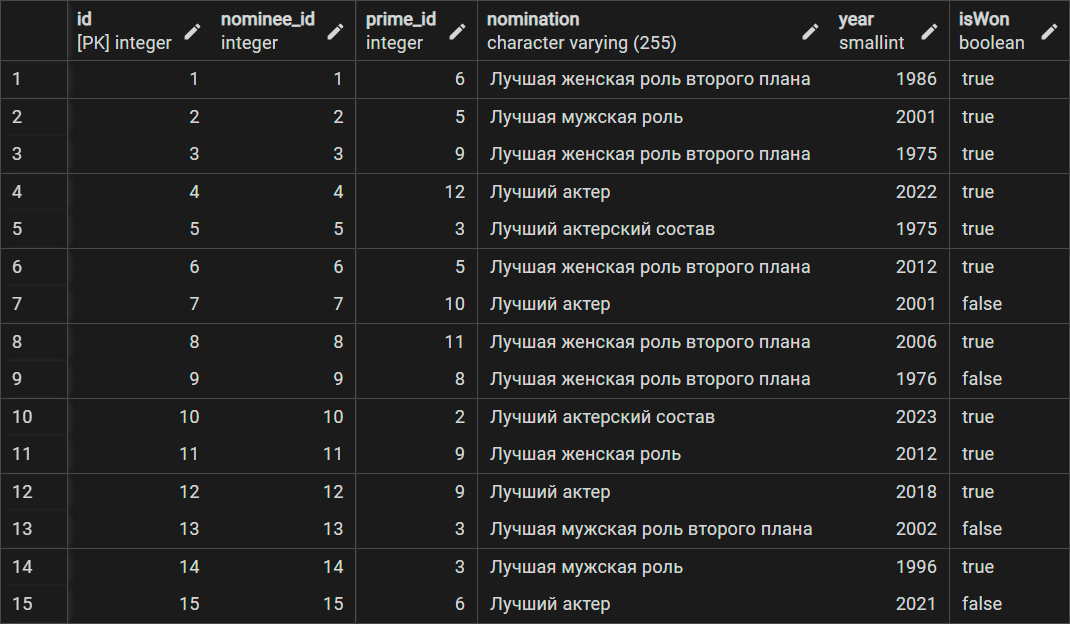
\includegraphics[scale=0.3,page=1]{table_inserts_examples/Prime_nominations}

	
	
	\item Фрагмент таблицы Cinemas
	
	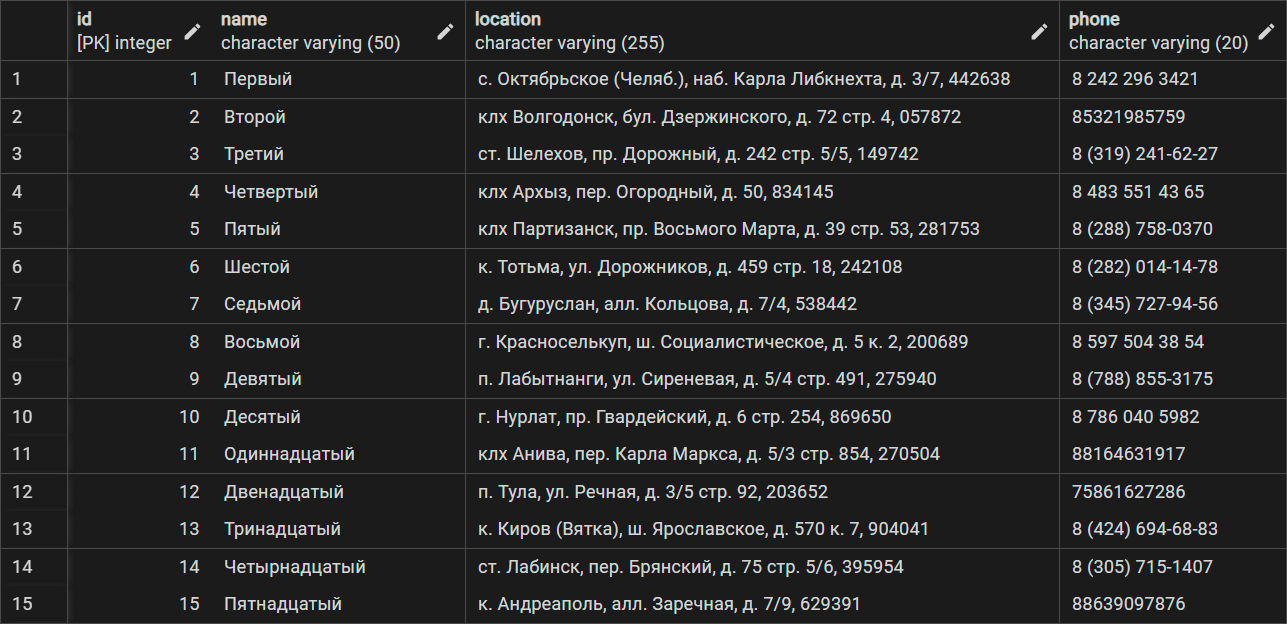
\includegraphics[scale=0.3,page=1]{table_inserts_examples/Cinemas}
	$\\$
	
	
	\item Фрагмент таблицы Halls
	
	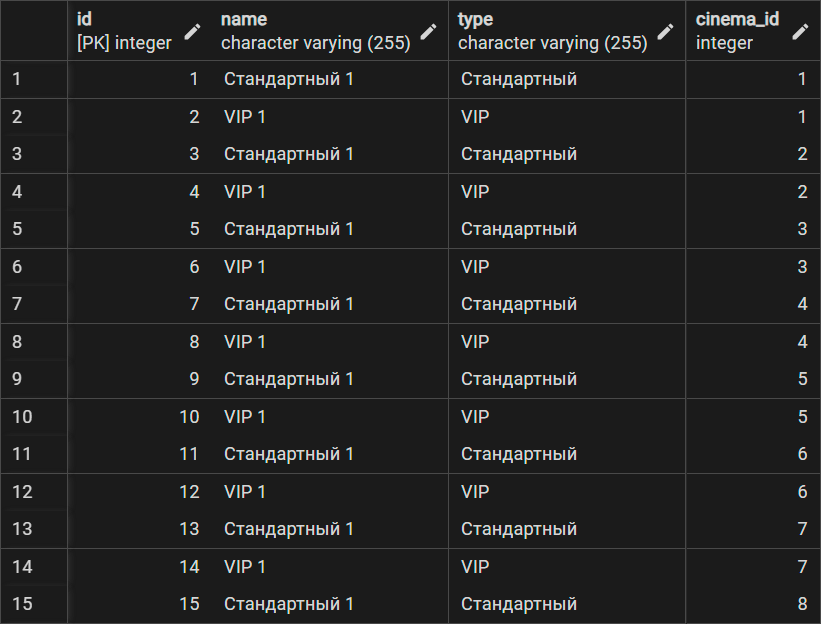
\includegraphics[scale=0.3,page=1]{table_inserts_examples/Halls}
	$\\$
	
	
	\item Фрагмент таблицы Sessions
	
	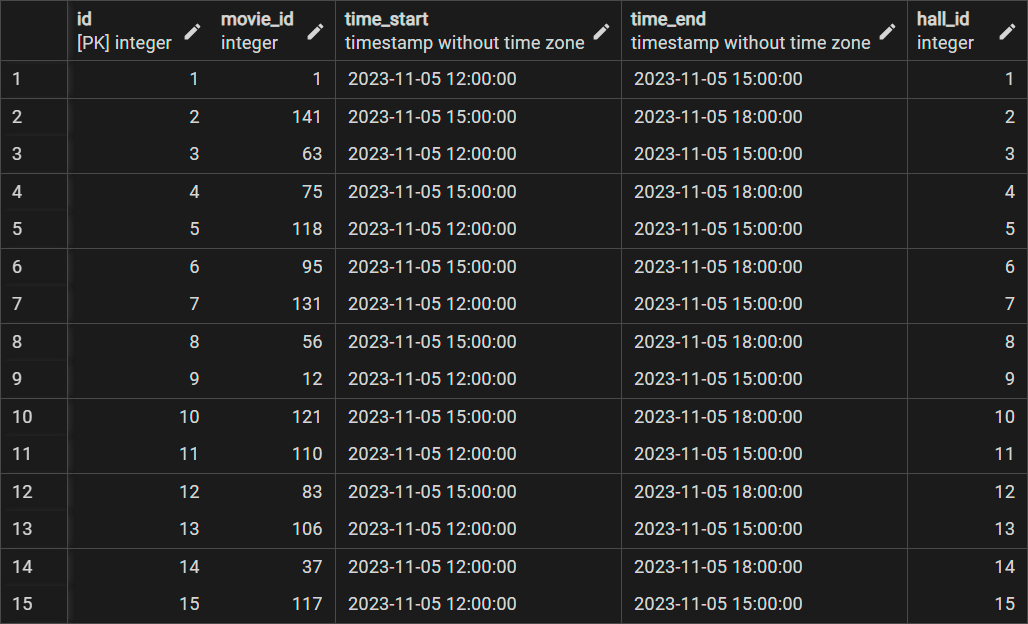
\includegraphics[scale=0.3,page=1]{table_inserts_examples/Sessions}
	$\\$

	
	\item Фрагмент таблицы Seats
	
	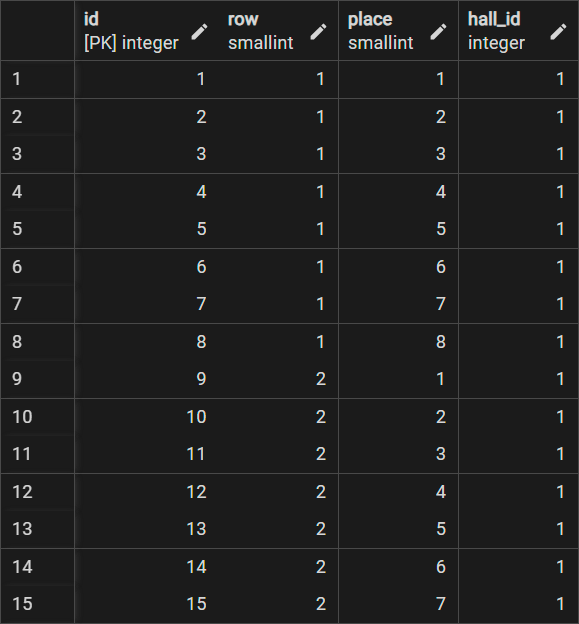
\includegraphics[scale=0.32,page=1]{table_inserts_examples/Seats}
	$\\$
	
	
	\item Фрагмент таблицы Customers
	
	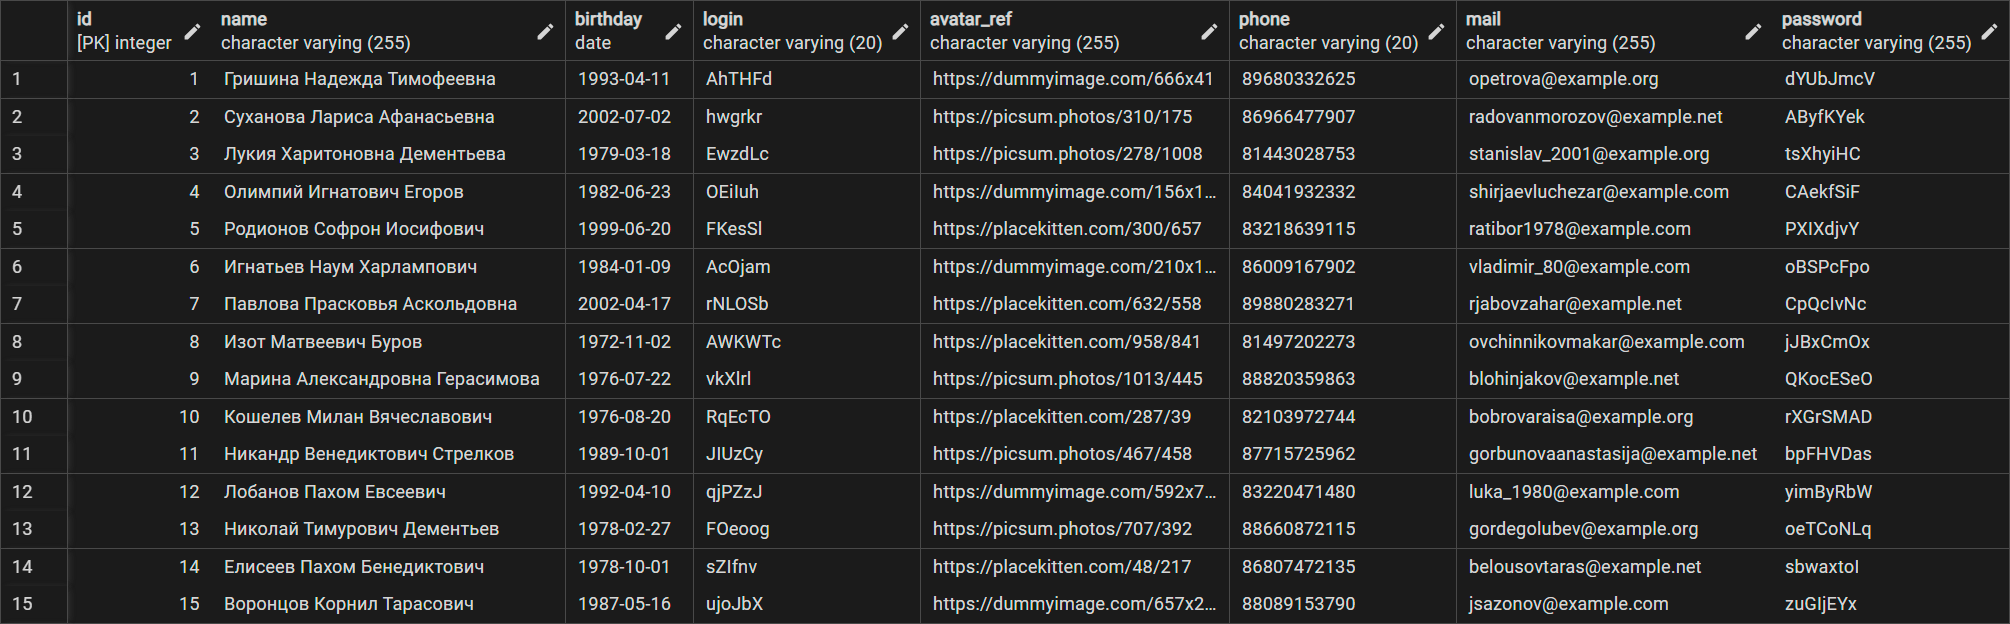
\includegraphics[scale=0.24,page=1]{table_inserts_examples/Customers}
	$\\$
	
	
	\item Фрагмент таблицы Orders
	
	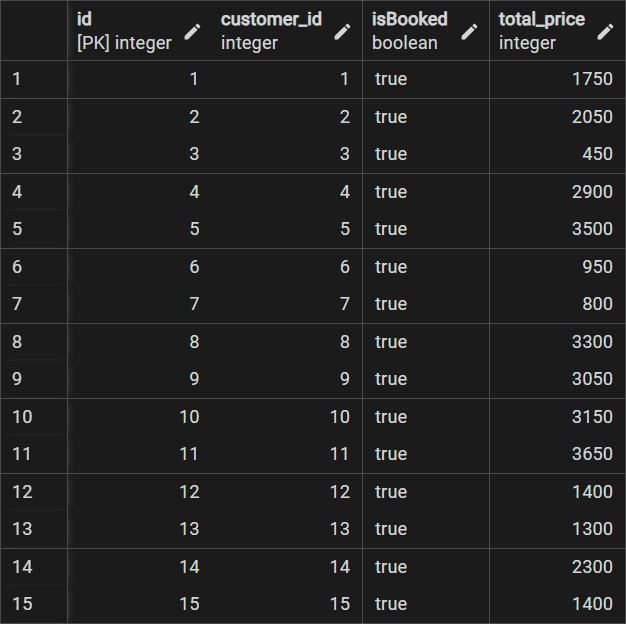
\includegraphics[scale=0.32,page=1]{table_inserts_examples/Orders}
	$\\$
	
	
	\item Фрагмент таблицы Payment
	
	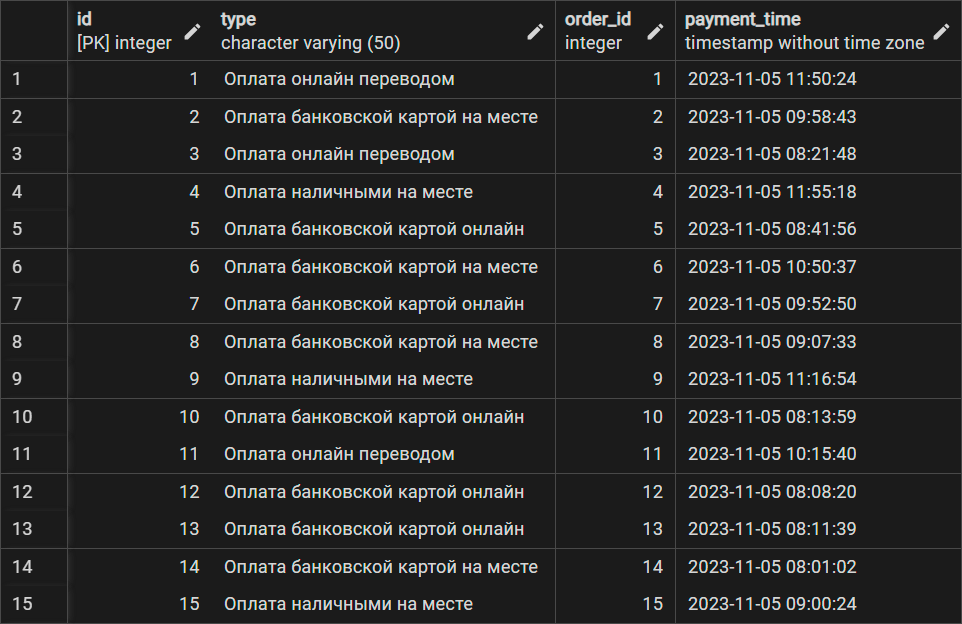
\includegraphics[scale=0.3,page=1]{table_inserts_examples/Payment}
	$\\$
	
	
	\item Фрагмент таблицы Tickets
	
	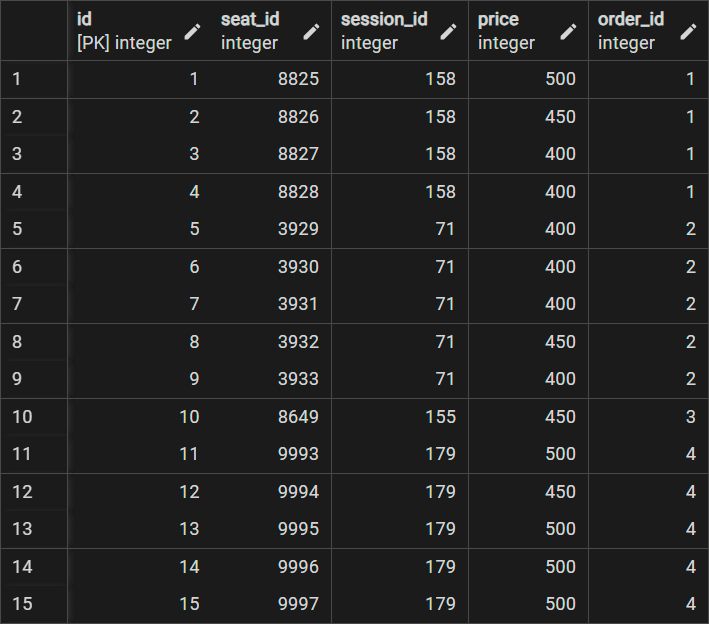
\includegraphics[scale=0.3,page=1]{table_inserts_examples/Tickets}
	$\\$
	
	
	\item Таблица Cinemas\_positions
	
	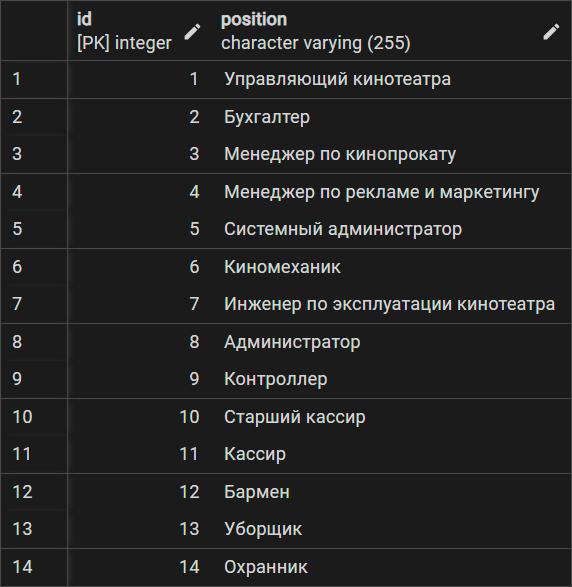
\includegraphics[scale=0.3,page=1]{table_inserts_examples/Cinemas_positions}
	$\\$
	
	
	\item Фрагмент таблицы Staff
	
	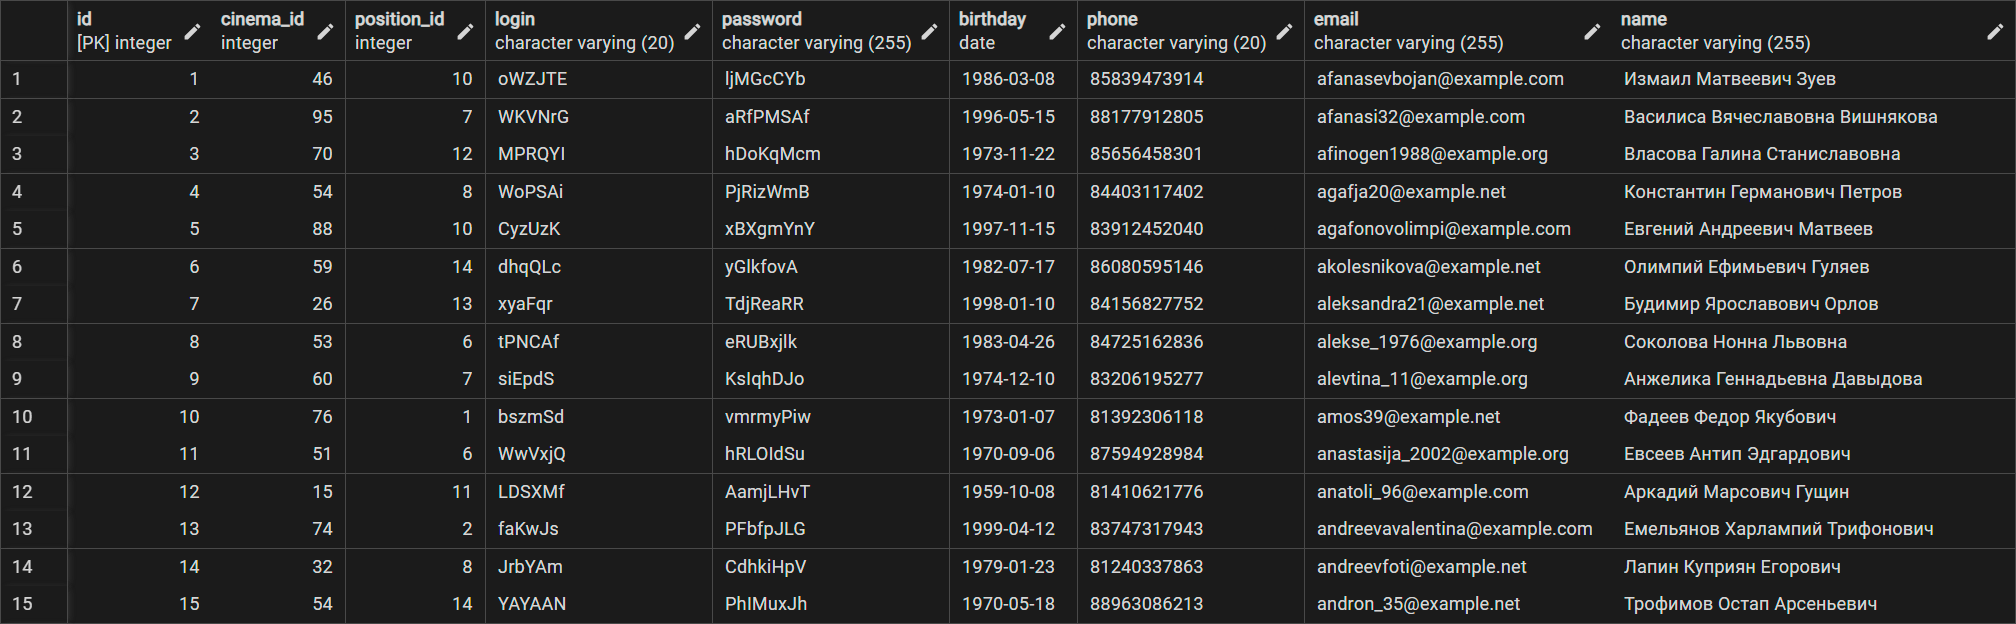
\includegraphics[scale=0.24,page=1]{table_inserts_examples/Staff}
	
	
		
	\end{itemize}
	
	\newpage
	
	\section{Выполнение запросов}\label{sec:-3}

	\begin{enumerate} 
		\item Получить неоплаченные заказы и тех, кто не оплатил
			\begin{lstlisting}[style=vscode-dark, language=SQL, label={lst:sql20}]
				SELECT o.id, c.name
				FROM "public.Orders" o
				JOIN "public.Customers" c ON c.id = o.customer_id
				JOIN "public.Payment" p ON o.id = p.order_id
				WHERE p.payment_time IS NULL;
			\end{lstlisting}
  			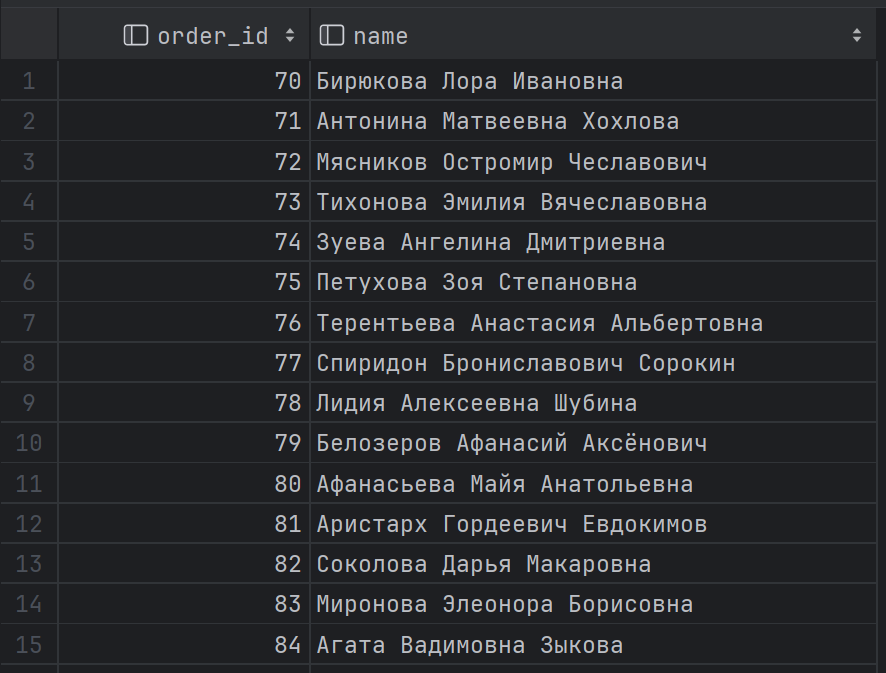
\includegraphics[scale=0.6,page=1]{queries/q1}
			$\\$
  
  
		\item Получить все сеансы на день в кинотеатре
			\begin{lstlisting}[style=vscode-dark, language=SQL, label={lst:sql21}]
				SELECT m.id, m.name, m.duration, s.time_start, h.type
				FROM "public.Sessions" s
				JOIN "public.Movies" m on m.id = s.movie_id
				JOIN "public.Halls" h on s.hall_id = h.id
				JOIN "public.Cinemas" c on h.cinema_id = c.id
				WHERE s.time_start::date = '2023-11-05'
    			AND c.name = 'Четвертый';
			\end{lstlisting}
			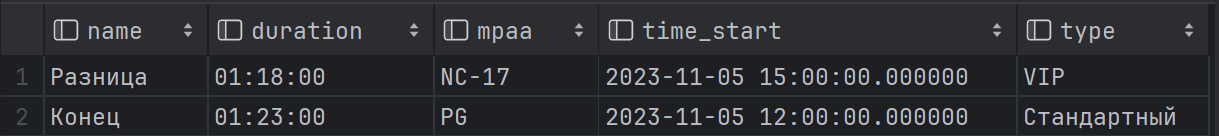
\includegraphics[scale=0.6,page=1]{queries/q2}
			$\\$

		\item Получить почты клиентов, родившихся в 90е (для какой-нибудь рассылки)
			\begin{lstlisting}[style=vscode-dark, language=SQL, label={lst:sql22}]
				SELECT c.mail, c.birthday
				FROM "public.Customers" c
				WHERE c.mail IS NOT NULL
					AND c.birthday < '2000-01-01'
					AND c.birthday >= '1990-01-01';
			\end{lstlisting}
			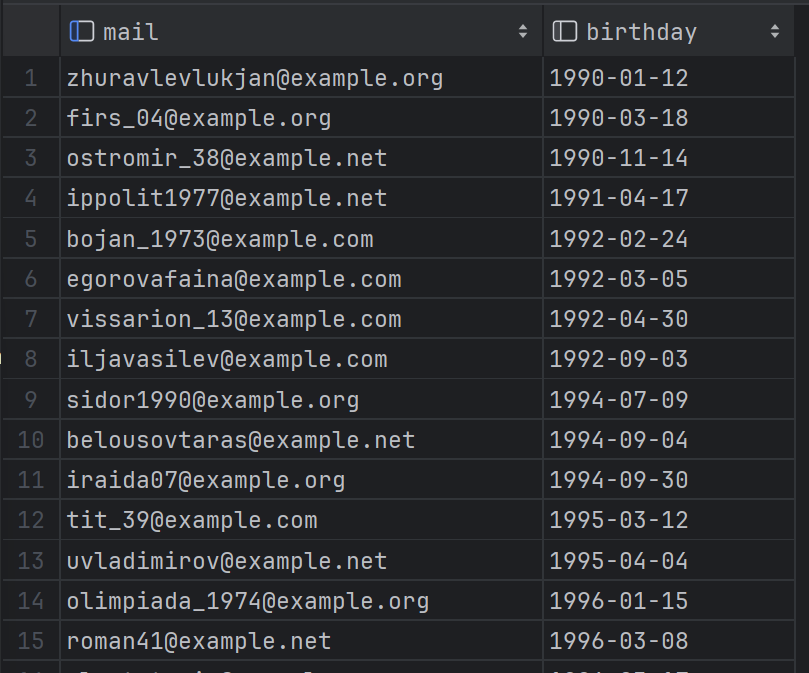
\includegraphics[scale=0.6,page=1]{queries/q3}
			$\\$

		\item Получить всех актеров какого-нибудь фильма, сортированных по убыванию возраста
			\begin{lstlisting}[style=vscode-dark, language=SQL, label={lst:sql23}]
				SELECT fcm.id, fcm.name, fcm.birthday
				FROM "public.Film_crew_members" fcm
				JOIN "public.Films_positions" fp ON fcm.id = fp.member_id
				JOIN "public.Movies" m ON fp.movie_id = m.id
				WHERE m.name = 'Тип семейства'
					AND fp.name = 'Актер'
				ORDER BY fcm.birthday;
			\end{lstlisting}
			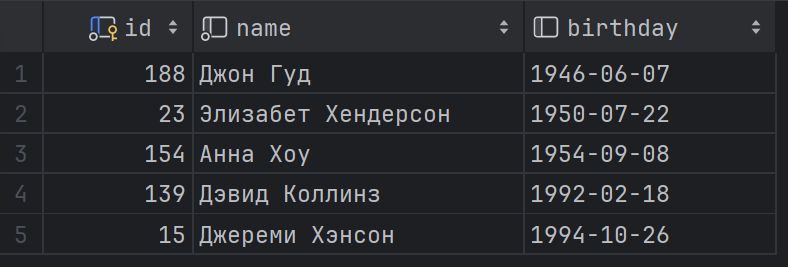
\includegraphics[scale=0.6,page=1]{queries/q4}
			$\\$

		\item Получить фильмы, которые идут в этом кинотеатре в жанре Мультфильмы
			\begin{lstlisting}[style=vscode-dark, language=SQL, label={lst:sql24}]
				SELECT m.id, m.name, s.time_start
				FROM "public.Sessions" s
				JOIN "public.Movies" m ON m.id = s.movie_id
				JOIN "public.Movies_genres" mg ON m.id = mg.movie_id
				JOIN "public.Genres" g ON mg.genres_id = g.id
				JOIN "public.Halls" h ON s.hall_id = h.id
				JOIN "public.Cinemas" c ON h.cinema_id = c.id
				WHERE s.time_start::date = '2023-11-05'
					AND g.name = 'Мультфильмы'
					AND c.name = 'Одиннадцатый';
			\end{lstlisting}
			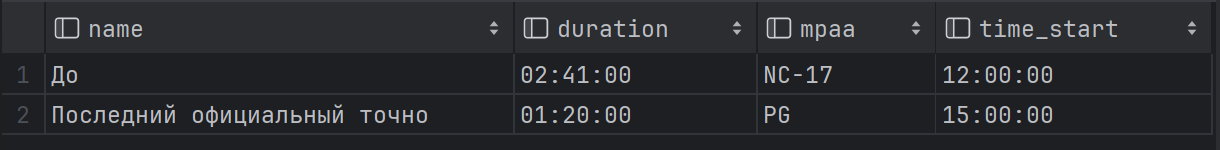
\includegraphics[scale=0.6,page=1]{queries/q5}
			$\\$

		\item Получить количество занятых мест в зале на сеансе
			\begin{lstlisting}[style=vscode-dark, language=SQL, label={lst:sql25}]
				SELECT COUNT(t.id)
				FROM "public.Tickets" t
				JOIN "public.Sessions" s ON t.session_id = s.id
				JOIN "public.Movies" m ON m.id = s.movie_id
				JOIN "public.Halls" h ON s.hall_id = h.id
				JOIN "public.Cinemas" c on h.cinema_id = c.id
				JOIN "public.Orders" o ON t.order_id = o.id
				WHERE m.name = 'Мировая сумка-машина'
					AND s.time_start::date = '2023-11-05'
					AND c.name = 'Сотый'
					AND h.type = 'VIP'
					AND o."isBooked" = True;
			\end{lstlisting}
			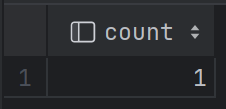
\includegraphics[scale=0.6,page=1]{queries/q6}
			$\\$

		\item Узнать сумму цен на забронированные, но не проданные билеты
			\begin{lstlisting}[style=vscode-dark, language=SQL, label={lst:sql26}]
				SELECT SUM(t.price)
				FROM "public.Tickets" t
				JOIN "public.Orders" o ON t.order_id = o.id
				JOIN "public.Payment" p ON o.id = p.order_id
				WHERE o."isBooked" = True
					AND p.payment_time IS NULL;
			\end{lstlisting}
			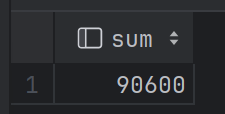
\includegraphics[scale=0.6,page=1]{queries/q7}
			$\\$

		\item Обновление пароля клиента по почте
			\begin{lstlisting}[style=vscode-dark, language=SQL, label={lst:sql27}]
				UPDATE "public.Customers"
				SET password = 'updatedpass'
				WHERE mail = 'bobrovaraisa@example.org';
			\end{lstlisting}
			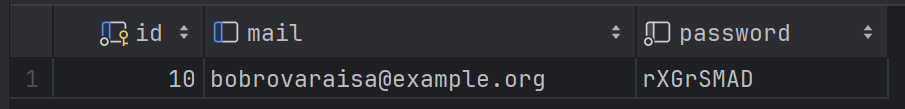
\includegraphics[scale=0.6,page=1]{queries/q8before}
			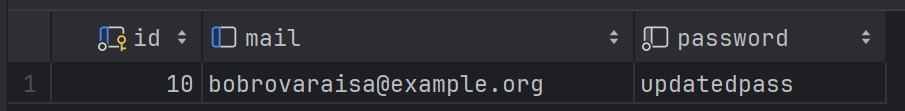
\includegraphics[scale=0.6,page=1]{queries/q8after}
			$\\$

		\item Удаление всех сеансов с этим фильмом
			\begin{lstlisting}[style=vscode-dark, language=SQL, label={lst:sql28}]
				DELETE FROM "public.Sessions" s
				WHERE s.movie_id = (SELECT m.id FROM "public.Movies" m
                           			 WHERE m.name = 'Помнить'
									);
			\end{lstlisting}
			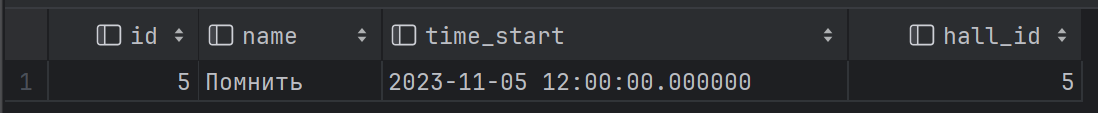
\includegraphics[scale=0.6,page=1]{queries/q9before}\\
			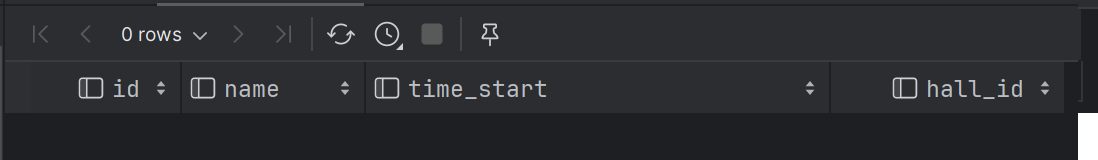
\includegraphics[scale=0.6,page=1]{queries/q9after}
			$\\$

		\item Вывести фильмы в порядке убывания количества сеансов в определённый день
			\begin{lstlisting}[style=vscode-dark, language=SQL, label={lst:sql29}]
				SELECT m.id, m.name, COUNT(s.id) AS session_count
				FROM "public.Movies" m
				JOIN "public.Sessions" s ON m.id = s.movie_id
				WHERE s.time_start::date = '2023-11-05'
				GROUP BY m.id
				ORDER BY session_count DESC;
			\end{lstlisting}
			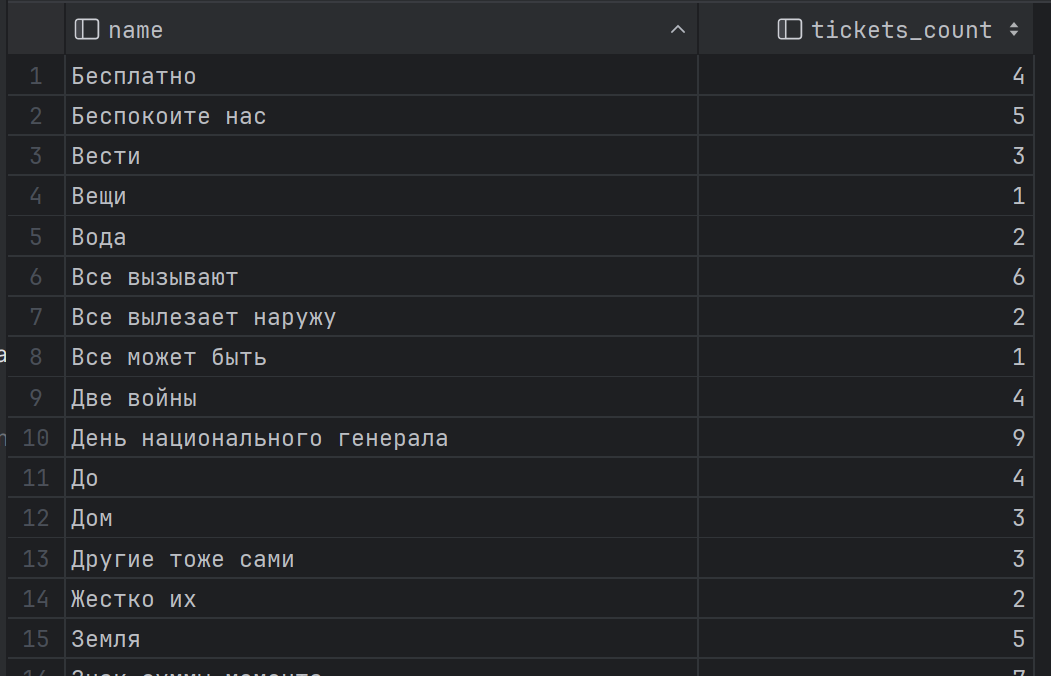
\includegraphics[scale=0.6,page=1]{queries/q10}
			$\\$


		\item Вывести отношение билетов, проданных онлайн, ко всем проданным билетам
			\begin{lstlisting}[style=vscode-dark, language=SQL, label={lst:sql32}]
				WITH paid_total AS (
					SELECT count(t.id) AS count
					FROM "public.Tickets" t
					JOIN "public.Orders" o ON o.id = t.order_id
					JOIN "public.Payment" p ON o.id = p.order_id
						WHERE p.payment_time IS NOT NULL
				),
				paid_online AS (
					SELECT count(t.id) AS count
					FROM "public.Tickets" t
					JOIN "public.Orders" o ON o.id = t.order_id
					JOIN "public.Payment" p ON o.id = p.order_id
					WHERE p.payment_time IS NOT NULL
						AND (p.type = 'Оплата онлайн переводом'
						OR p.type = 'Оплата банковской картой онлайн')
				)
				SELECT paid_online.count AS online_count, paid_total.count AS total_count,
    					100 * paid_online.count / paid_total.count AS online_percentage
				FROM paid_total, paid_online
			\end{lstlisting}
			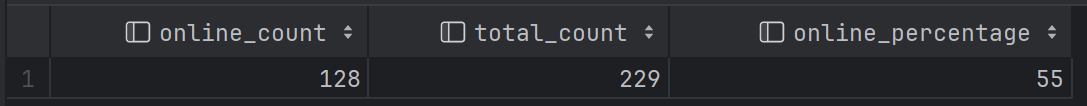
\includegraphics[scale=0.6,page=1]{queries/q11}
			$\\$


		\item Получить средний возраст зрителей фильмов с рейтингом R
			\begin{lstlisting}[style=vscode-dark, language=SQL, label={lst:sql30}]
				SELECT avg(age(c.birthday))
				FROM "public.Customers" c
				JOIN "public.Orders" o ON c.id = o.customer_id
				JOIN "public.Tickets" t ON o.id = t.order_id
				JOIN "public.Sessions" s ON t.session_id = s.id
				JOIN "public.Movies" m ON s.movie_id = m.id
				JOIN "public.Payment" p ON o.id = p.order_id
				WHERE m.mpaa = 'R'
   					 AND p.payment_time IS NOT NULL;
			\end{lstlisting}
			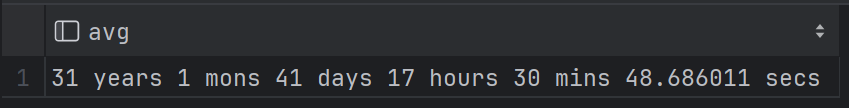
\includegraphics[scale=0.6,page=1]{queries/q12}
			$\\$


		\item Получить выручку по месяцам этого года
			\begin{lstlisting}[style=vscode-dark, language=SQL, label={lst:sql31}]
				SELECT extract(month from p.payment_time), sum(o.total_price)
				FROM "public.Orders" o
				JOIN "public.Payment" p On o.id = p.order_id
				WHERE p.payment_time IS NOT NULL
					AND extract(year from p.payment_time) = extract(year from current_timestamp)
				GROUP BY extract(month from p.payment_time);
			\end{lstlisting}
			\includegraphics[scale=0.6,page=1]{queries/q13}
			$\\$


		\item Процент фильмов, которые есть в базе, но не были в прокате
			\begin{lstlisting}[style=vscode-dark, language=SQL, label={lst:sql35}]
				WITH movies_null AS (
					SELECT count(m.id) AS count
					FROM "public.Movies" m
					LEFT JOIN "public.Sessions" s on m.id = s.movie_id
					WHERE s.id is NULL
				),
					movies_all AS (
					SELECT count(*) AS count
					FROM "public.Movies"
				)
				SELECT 100 * movies_null.count / movies_all.count AS percentage
				FROM movies_null, movies_all;
			\end{lstlisting}
			\includegraphics[scale=0.6,page=1]{queries/q14}
			$\\$


		\item Поиск всех подкатегорий
			\\Инициализация таблицы
		\begin{lstlisting}[style=vscode-dark, language=SQL, label={lst:sql33}]

			CREATE TABLE categories (
				id INT PRIMARY KEY,
				name VARCHAR(100),
				parent_id INT REFERENCES categories(id)
			);

			INSERT INTO categories (id, name, parent_id)
			VALUES (1, 'Electronics', NULL),
				   (2, 'Computers', 1),
				   (3, 'Laptops', 2),
				   (4, 'Gaming Laptops', 3),
				   (5, 'Ultrabooks', 3),
				   (6, 'Desktops', 2),
				   (7, 'Phones', 1),
				   (8, 'Smartphones', 7),
				   (9, 'Feature Phones', 7);
		\end{lstlisting}
		Поиск всех подкатегорий для категории Computers
		\begin{lstlisting}[style=vscode-dark, language=SQL, label={lst:sql34}]
			WITH RECURSIVE r AS (
				SELECT id, name, parent_id
				FROM categories
				WHERE name = 'Computers'

				UNION

				SELECT categories.id, categories.name, categories.parent_id
				FROM categories
				JOIN r ON categories.parent_id = r.id
			)
			SELECT r.name
			FROM r
			WHERE r.name != 'Computers'
			ORDER BY r.id;
		\end{lstlisting}
		\includegraphics[scale=0.6,page=1]{queries/q_rec}
		$\\$
	\end{enumerate}

\end{document}
